\documentclass[12pt]{article}

\usepackage{amssymb,amsmath,amsfonts,verbatim,graphicx,titlesec,float,setspace,soul,fancyhdr,fullpage,palatino}
\usepackage[usenames,dvipsnames]{color}
\usepackage[hidelinks]{hyperref}
\usepackage{subcaption}
\usepackage{amsthm}
\newtheorem{theorem}{Theorem}

\pagestyle{fancyplain}

\titleformat*{\section}{\large\bfseries}
\titleformat*{\subsection}{\normalsize\bfseries}
\titleformat*{\subsubsection}{\normalsize\bfseries}

% document parameters
\setlength{\textheight}{9in}
\setlength{\parindent}{0pt}
\setlength{\parskip}{8pt}
\setlength{\parindent}{0.in}
\setlength{\parskip}{0.1in}
\setlength{\topmargin}{-0.4in}
\setlength{\headsep}{0.4in}

\newcommand{\sech}[0]{\mathrm{sech}}
\newcommand{\pd}[0]{\partial}
\newcommand{\dd}[0]{\mathrm{d}}
\newcommand{\AG}[1]{{\color{Green} (#1)}}
\newcommand{\mc}[1]{\mathcal{#1}}
\numberwithin{equation}{section}

\title{Project summary: asymptotic reductions of the steady KP equation}
\author{\vspace{-1in}}
\date{\vspace{-1in}}
\begin{document}

\maketitle
\tableofcontents
\pagebreak

\section{Introduction}
\subsection{KP Whitham system}

Consider the  Kadomstev-Petviashvili (KP)
equation \cite{kp1970}
\begin{align}
  \label{eq:1}
  (u_t + 6 uu_x + u_{xxx})_x + \sigma u_{yy} &= 0,
\end{align}\label{originalKP}
where $\sigma = -1$ is called KPI (strong surface tension) and
$\sigma = +1$ is KPII (strong gravity). The linear dispersion relation for \eqref{originalKP} is
$\omega = (6u_-+\sigma q^2)k-k^3$, where $k$ and $l$ are the local
wavenumbers in the $x$ and $y$ directions, respectively, and $q=l/k$,
i.e., the phase is $\theta = k x + l y - \omega t$. The KP equation
admits exact nonlinear, periodic traveling wave solutions of the form
\begin{align}
    u (x,y,t) = r_1 - r_2 + r_3 +2(r_2-r_1)\text{cn}^2(2\theta K_m;m), \hspace{3mm}  v(x,y,t)=  qu+p, \label{exactsol}
\end{align}
where $ u_y = v_x$, $K_m=K(m)$ is the complete elliptic integral of the first kind, and 
and
\begin{align}
    m = \frac{r_2-r_1}{r_3-r_1} \label{mrule}
\end{align}
is the elliptic parameter. The solution is therefore determined by the
five parameters $r_1,r_2,r_3,q$ and $p$. The following relationships
hold:
\begin{subequations}
\begin{align}
    k &= \sqrt{r_3-r_1}/2K_m \label{keqxn} \\
    l &= qk \label{leqxn}\\
    \omega &= (V+\sigma q^2)k \\
    V&= \frac{\omega}{k} - \sigma q^2 = 2(r_1+r_2+r_3).
\end{align}
\end{subequations}

In \cite{ablowitz2017whitham}, The KP-Whitham system (KPWS) is obtained in terms of the modulation variables $r_1,r_2,r_3,q, \omega,$ and $p$. 

Now, we consider the case in which there is no modulation in time; that is, $\omega_x = \omega_y = 0$, to reduce to the five variables $r_1,r_2,r_3,q$ and $p$. In \cite{biondini2023two} this is called the XY system, because $\omega$ is constant and the system is modulated only in $x$ and $y$.

We can use the dispersion relation for the KP equation, 
\begin{align}
    \omega = (V + \sigma q^2)k
\end{align}
with zero mean flow, $u_- = 0$, and constant frequency modulation to obtain the following relation for $q$:
\begin{align}
    q & =  \pm \sqrt{\sigma\left(\frac{\omega}{k}-2(r_1+r_2+r_3)\right)} \label{qexn}
\end{align}
and we can use \eqref{qexn} to eliminate $q$ as a dependent variable. This process requires a choice of sign for $q$. We can then make a change of dependent variable to $[r_1,r_2,r_3,\omega,p]^T$ and eliminate the fourth equation to obtain the the four-variable system \eqref{vector eq for statKPWS} in $r_1,r_2,r_3$, and $p$. We can do this because all derivatives of $\omega$ are zero, resulting in a system where the fourth columns and fourth rows in both matrices are all zero. 
\begin{align}
    A\frac{\partial \textbf{p}}{\partial x} + B\frac{\partial \textbf{p}}{\partial y} =0, \label{vector eq for statKPWS}
\end{align}
where $\textbf{p} = [r_1,r_2,r_3,p]^T$, and 
\begin{subequations}
{\tiny
\begin{align}
       A &= \left[\begin{array}{cccc}
        q((c_1+1)v_++q^2(-\sigma)+v_+) & -(c_1+c_2-1)v_+q & (c_2+1)v_+q & -q^2 \sigma  \\
         (c_1 + 1)v_2q & -q((c_1+c_2-1)v_2+q^2\sigma -V_2) & (c_2+1)v_2q & -q^2\sigma \\
         (c_1+1)v_3q & -(c_1+c_2-1)v_3q & q((c_2+1)v_3q + q^2(-\sigma)+V_3) ^ -q^2\sigma \\
         -\sigma(c_1+1)v_5-((\alpha-1)q^2) & \sigma(c_1+c_2-1)v_5 & \alpha q^2 -\sigma(c_2+1)v_5 & q
    \end{array}\right] \label{a4p} \\
     B &= \left[\begin{array}{cccc}
        2\sigma q^2 -(c_1+1)v_+ & (c_1+c_2-1)v_+ & -((c_2+1)v1) & q\sigma \\
        -((c_1+1)v_2) & 2 \sigma q^2 + (c+1+c_2-1)v_2 & -((c_2+1)v_+) & q\sigma \\
        -((c_1+1)v_3) & (c_1+c_2-1)v_3 & 2\sigma q^2 -(c_2+1)v_3 & q\sigma \\
        (\alpha -1)q & 0 & -\alpha q & 0
    \end{array}\right] \label{b4p}
\end{align}
}    
\end{subequations}
(The above are derived in detail in \cite{biondini2023two}). In the above matrices, 
\begin{align}
    v_+ = V-2a\frac{K_m}{K_m-E_m}, \hspace{3mm} V_2 = V-2a\frac{(1-m)K_m}{E_m-(1-m)K_m}, \hspace{3mm} V_3 = V+2a\frac{(1-m)K_m}{mE_m}
\end{align}
and $a = 2(r_2-r_1)$ is the cnoidal wave amplitude, with coefficients
\begin{subequations}
\begin{align}
    v_+&=\frac{V}{6} + \frac{b}{3m}\frac{(1+m)E_m-K_m}{K_m-E_m}, \hspace{3mm} v_2 = \frac{V}{6} + \frac{b}{3m}\frac{(1-m)^2K_m-(1-2m)E_m}{E_m-(1-m)K_m}, \\
    v_3 &= \frac{V}{6} + \frac{b}{3m}\frac{(2-m)E_m - (1-m)K_m}{E_m}, \hspace{3mm} v_4 = \frac{2mE_m}{E_m-(1-m)K_m}, \\
    v_5 &= r_1-r_2+r_3, \hspace{3mm} \alpha = \frac{E_m}{K_m}
\end{align}
\end{subequations}
and
\begin{align}
    c_1 = \frac{\omega(E_m-K_m)}{16mk^3K_m^3}, \hspace{3mm} c_2 = \frac{\omega E_m}{16k^2K_m^3(1-m)}.
\end{align}



\subsection{Steady reduction}
In this work, we will examine steady reductions of of the KP system. The steady KP equation is given by 
\begin{align}
    (6uu_x + u_{xxx})_x + \sigma u_{yy} &= 0 .
    \label{statKP}
\end{align}
Or, in evolution form, by
\begin{subequations}
    \begin{align}
        u_y &= v_x \\
        v_y &= -\sigma(6uu_x + u_{xxx})
    \end{align} \label{steady KP evolution}
\end{subequations}
where we have defined the new dependent variable $v(x,y)$ such that $v_x = u_y$. We are therefore able to interpret $(u,v)$ as an irrotational velocity field in two dimensions.

The KP Whitham system for the steady case is given by \eqref{vector eq for statKPWS} with a few modifications. Specifically, we assume that $\omega = 0$ (If we take $\omega = \rm const$, we have time-varying flow that is not modulated in time). This means that, from \eqref{qexn},
\begin{align}
    q  &=\pm \sqrt{-2\sigma(r_1+r_2+r_3)} \label{qexn, omega=0} 
\end{align}
and $c_1 = c_2=0$. 

\subsection{Equivalence to Boussinesq equation} \label{sec: equiv to bouss}
Consider the Boussinesq equation for undirectional fluid flow with velocity $U$:
\begin{align}
  U_{tt}-U_{xx} + (U^2)_{xx} + \sigma U_{xxxx} = 0
    \label{boussinesq}
\end{align}
where $\sigma = 1$ gives the "good" Boussinesq equation (gBq), and $\sigma = -1$ gives the "bad" Boussinesq equation (bBq). \eqref{boussinesq} is equivalent to \eqref{statKP} under the transformation
\begin{align}
    U = 3u + \frac{1}{2}; \; u = \frac{1}{3}\left(U - \frac{1}{2} \right), \; t = y.\label{trans bouss to kp}
\end{align}
That is, gBq is equivalent to steady KPII, and bBq is equivalent to steady KPI.

If we define the new dependent variable $V$ such that $V_x = U_t$, then we can also write the Boussinesq equation in evolution form:
\begin{subequations}
    \begin{align}
        U_t &= V_x \\
        V_t &= U_x - \left(U^2\right)_x - \sigma U_{xxx}
    \end{align} \label{boussinesq evolution}
\end{subequations}

\subsection{Symmetries} \label{sec: symmetries}
The steady KP equation also exhibits useful symmetries. Suppose that we start with \eqref{statKP} and take $x \to -x$. Then each $x$ derivative gains a negative sign, and we have 
\begin{align*}
    -(-6uu_x - u_{xxx})_x + \sigma u_{yy} &= 0,
\end{align*}
which, when simplified, gives
\begin{align*}
    (6uu_x + u_{xxx})_x + \sigma u_{yy} &= 0,
\end{align*}
the same as \eqref{statKP}. Therefore \eqref{statKP} is invariant under the transformation $x \to -x$. Similarly, it is easy to see that \eqref{statKP} is invariant under the transformation $y \to -y$. 

Now suppose that we start with the disperionless limit of steady KPII, discussed in section \ref{sec: disp limit}:
\begin{align}
    (6uu_x)_x + u_{yy} &= 0, 
    \label{statKPII}
\end{align}
and we take $u \to -u$. Then we have
\begin{align}
    (6uu_x)_x - u_{yy} &= 0, 
\end{align}
which is the dispersionless limit of steady KPI.

\section{Dispersionless limit of steady KP} \label{sec: disp limit}
First we consider the dispersionless limit of \eqref{statKP}. We can find this by taking $x \to \varepsilon x$, where $0 <\varepsilon \ll 1$, and examining the leading order problem. This is
\begin{align}
     (6uu_x)_x + \sigma u_{yy} &= 0. \label{KP2Dstatdisp}
\end{align}


%%%%%%%%%%%%%%%%%%%%%%%%%%%%%%%%%%%%%%%%%%%%%%%%%%%%%%%%%%%%%%%%%%%%%%%%%%%%%%%%%%%%%%%%%%%%%%%%%%%%%%%%%%%
\begin{figure}
    \centering
    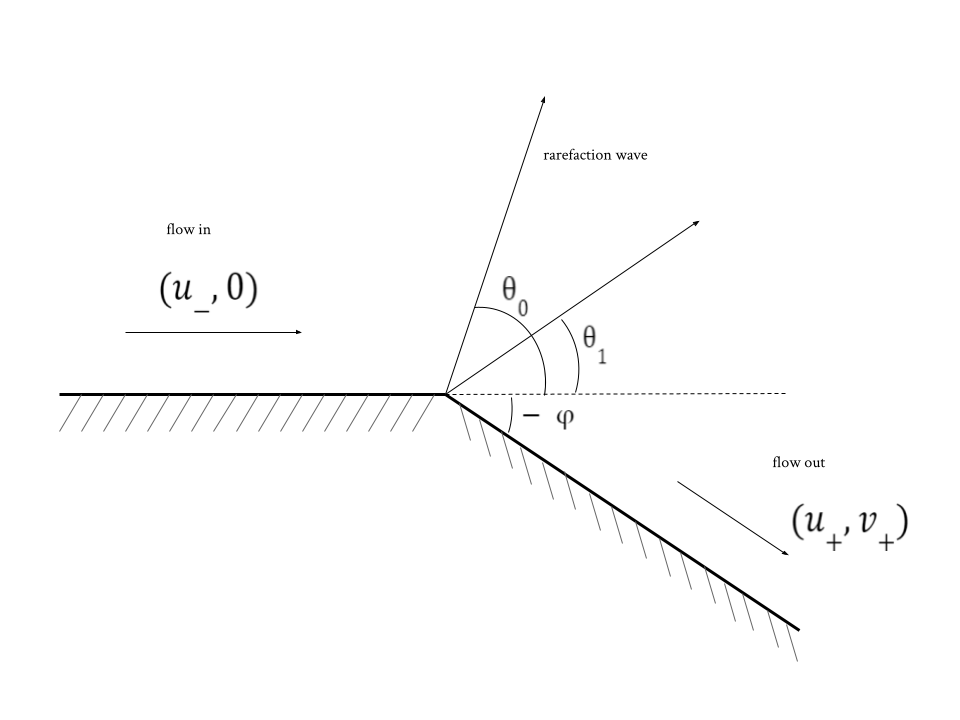
\includegraphics[width = 0.7\textwidth]{figures/Stationary KP diagram.png}
    \caption{Flow around a corner creating a stationary rarefaction wave, described by system \ref{disp kp1 evolution}; that is, system \ref{KP2Dstatdisp} with $\sigma = -1$. However, due to the symmetry $u \mapsto -u$, to represent the case $\sigma = +1$ we need only take the mirror image (about the vertical axis) of the above figure. Diagram is editable and accessible at \href{https://docs.google.com/drawings/d/1szWVgUYcond4bVDgIpK8ZXEmS2uC1-2WPGRDoJfGp7Y/edit?usp=sharing}{\bf this link}.}
    \label{fig:stationarydiagram}
\end{figure}
Because of the symmetry discussed in section \ref{sec: symmetries}, we can easily obtain solutions to KPII from solutions to KPI and vice versa by taking $u \to -u$. We choose the $\sigma = -1$ (KPI) case; that is,
\begin{align}
    (6uu_x)_x - u_{yy}=0\label{minus1}
\end{align}
which can be given in evolution form as
\begin{align}
\begin{array}{rl}
    u_y &= v_x \\
     v_y &= 6uu_x 
\end{array}.
\label{disp kp1 evolution}
\end{align}
where, as before, we have defined the dependent variable $v(x,y)$ such that $v_x = u_y$.

The dependent variables in \eqref{disp kp1 evolution} $(u,v)$ represent an irrotational velocity field; specifically, given a Riemann boundary condition
\begin{align}
    u(x,0) = \left\{\begin{array}{cc}
        u_- & x<0 \\
        u_+ & x>0
    \end{array}
    \right.
\end{align}
they describe flow around an expansive corner. Given an initial value $(u,v)=(u_-,0)$ and a corner with angle of depression $0<\varphi<\frac{\pi}{2}$ below the horizontal, said flow creates a standing wave with edges at angles $\theta_0$ and $\theta_1$, and an outward flow $(u,v)=(u_+,v_+)$ (see Figure \ref{fig:stationarydiagram}).


We obtain a self-similar solution to \ref{KP2Dstatdisp}, describing the rarefaction wave in terms of $u_-$ and $\varphi$. We use this solution and the geometry of the problem to find $\theta_0$, $\theta_1$, and $(u_+,v_+)$, and a one-to-one relationship between $\varphi$ and $u_+$.


%%%%%%%%%%%%%%%%%%%%%%%%%%%%%%%%%%%%%%%%%%%%%%%%%%%%%%%%%%%%%%%%%%%%%%%%%%%%%%%%%%%%%%%%%%%%%%%%%%%%%%%%%%5

\subsection{Hyperbolicity and Riemann invariants}
\label{sec:hyperbolicity}
First we rewrite \eqref{disp kp1 evolution} as a quasilinear matrix equation:
\begin{align}
\left[
    \begin{array}{cc}
        6u & 0 \\
        0 & -1
    \end{array}
    \right]
    \left[\begin{array}{c}
         u  \\
         v 
    \end{array}\right]_x + \left[\begin{array}{cc}
        0 & -1 \\
        1 & 0
    \end{array}\right]
    \left[\begin{array}{c}
         u  \\
         v 
    \end{array}\right]_y
    &= 
    \left[\begin{array}{c}
         0  \\
         0 
    \end{array}\right]
\end{align}
Let $A = \left[\begin{array}{cc}
    0 & -1 \\
    1 & 0
\end{array}\right]$. Then $A^{-1} = \left[\begin{array}{cc}
    0 & 1 \\
    -1 & 0
\end{array}\right]$. Multiplying by $A^{-1}$ on the left, we have
\begin{align}
    \left[\begin{array}{c}
         u  \\
         v 
    \end{array}\right]_y + 
    \left[\begin{array}{cc}
        0 & -1 \\
        -6 u & 0
    \end{array}\right]
    \left[\begin{array}{c}
         u  \\
         v 
    \end{array}\right]_x 
    &=
    \left[\begin{array}{c}
         0  \\
         0 
    \end{array}\right]
    \label{disp matrix system}
\end{align} 
Let $B = \left[\begin{array}{cc}
        0 & -1 \\
        -6u & 0
    \end{array}\right]$, with characteristic polynomial $f(\lambda) = \lambda^2 - 6u$. Denote the eigenvalues of $B$ as $\lambda_{1,2}$, the right eigenvectors as $r_{1,2}$, and the left eigenvectors as $\ell_{1,2}$. Then
    \begin{align}
        \lambda_{1,2} = \pm \sqrt{6u}, \; \ell_{1,2} = \left[
        \begin{array}{cc}
             \pm \sqrt{6u}\\
             -1
        \end{array}\right], \; 
        r_{1,2} =\left[
        \begin{array}{cc}
             1\\
             \pm \sqrt{6u}
        \end{array}\right]
        \label{lambda, l, r for disp limit}
    \end{align}
Let $s_{\pm}$ represent the Riemann invariants for the system. Taking the inner product of $\ell_{1,2}$ with \eqref{disp matrix system}, we have
\begin{subequations}
\begin{align}
    \mathrm{D} s_{1,2} = 0 &= \pm \sqrt{6u} \mathrm{D} u - \mathrm{D} v,
\end{align}
where $D$ is the differential operator $\mathrm{D} = \pd_y + \lambda_i\pd_x$. Integrating once, we can solve for the Riemann invariants:
\begin{align}
    s_{1,2} &= -v \pm\frac{1}{9}(6u)^{3/2} \label{riemanninvariants}
\end{align}
\end{subequations}
Along the characteristics, $$\frac{\dd x}{\dd y} = \lambda_{1,2} = \pm \sqrt{6u}.$$
Thus, from the chain rule, $(s_{\pm})_y + \lambda_{1,2} (s_{\pm})_x = \dd s_{\pm}/\dd y=0$, and we obtain the following system of PDEs for $s_{\pm}:$
\begin{subequations}
    \begin{align}
    (s_2)_y + \lambda_+(s_2)_x &= 0 \\
    (s_1)_y + \lambda_-(s_1)_x &= 0  \label{sPDE}
\end{align}
\end{subequations}

%\MH{express $\lambda_\pm$ in terms of $s_\pm$}
  


\subsection{Self-similar solutions}


 We seek self-similar
solutions to system \ref{sPDE}. Let $\xi = y/x$. Then
$\partial_x = -\frac{y}{x^2}\dd\xi$ and
$\partial_y = \frac{1}{x}\dd\xi$, and system \ref{sPDE} is reduced to
the following system of ODEs:
    \begin{align}
\left\{
\begin{array}{rl}
     \frac{\dd s_2}{\dd\xi}\left(1-\lambda_{+}\xi\right) &= 0. \\ 
     \frac{\dd s_1}{\dd\xi}\left(1-\lambda_{-}\xi\right) &= 0 
\end{array}\right.
    \label{sODE}
\end{align}
which we can solve by examining the following two cases:
\begin{enumerate}
    \item $s_2=s_0^+$ and $1-\lambda_- \xi = 0$, where $s_0^+$ is a constant. This is called a \textit{1-wave} because it corresponds to the characteristic $\frac{\dd x}{\dd y}=\lambda_-$, where $\lambda_-$ is the smaller eigenvalue.
     \item $s_1 = s_0^-$ and $1-\lambda_+\xi=0$, where $s_0^-$ is a constant. This is called the \textit{2-wave} because it corresponds to the characteristic $\frac{\dd x}{\dd y} = \lambda_+$, where $\lambda_+$ is the larger eigenvalue.
\end{enumerate}

%%%%Is this rationale for using the 2-wave correct? Or should it be the 1-wave?

Case 2 describes the rarefaction wave in Figure \ref{fig:stationarydiagram}, because the slope of the wave in the $x$-$y$ plane must be positive, corresponding to the positive eigenvalue. Solving for $u(x,y)$,
\begin{align}
    1-\lambda_+\xi &= 0 \nonumber \\
    1-\sqrt{6u}\frac{y}{x} &= 0 \nonumber \\
    u &= \frac{1}{6}\left(\frac{x}{y}\right)^2
    \label{ugen}
\end{align}
 Solving for $v(x,y)$,
\begin{align}
    s_1=s_0^-&=-v-\frac{1}{9}(6u)^{3/2} \nonumber \\ 
    v &= -\frac{1}{9}\left[\left(\frac{x}{y}\right)^2\right]^{3/2}-s_0^- \nonumber \\
    &=  -\frac{1}{9}\left|\frac{x}{y}\right|^3-s_0^-
    \label{vgen}
\end{align}
Denote the initial flow $(u_-,0)$ (see Figure \ref{fig:stationarydiagram}). To impose continuity of our solution, we now match this initial condition to Equations \ref{ugen} and \ref{vgen} by solving for $s_0^-$. Note that from \ref{ugen}, we have $x=\sqrt{6u_-}y$ on the left boundary of the wave. This gives
\begin{align}
    s_0^- &= -0-\frac{1}{9}\left|\frac{\sqrt{6u_-}y}{y}\right|^3 = -\frac{1}{9}(6u_-)^{3/2}
\end{align}
And we have expressions for $u$ and $v$ in the rarefaction wave
\begin{align}
    (u(x,y),v(x,y)) &= 
    \frac{1}{6}\left(\left(\frac{x}{y}\right)^2,\frac{2}{3}\left(-\left|\frac{x}{y}\right|^3+(6u_-)^{3/2}\right)\right) 
    \label{finaluv}
\end{align}
Finally, we use Equation \ref{finaluv} to find $(u_+,v_+)$ and the angles $\theta_0$ and $\theta_1$ in terms of $u_-$ and $\varphi$. Finding an expression for $\theta_0$, 
\begin{align}
    \tan \theta_0 &=\frac{y}{x} = \frac{1}{\sqrt{6u_-}} \nonumber \\
    \theta_0 &= \arctan\left(\frac{1}{\sqrt{6u_-}}\right)
\end{align}
Now, $v_+=\sin(-\varphi) = -\sin(\varphi)$ and $u_+ = \cos(-\varphi) = \cos(\varphi)$. We have the following system of equations for $u_+,v_+,\theta_1$:
\begin{align} 
\left\{
\begin{array}{rl}
     \tan \theta_1 &= \frac{1}{\sqrt{6u_+}} \\
     \tan \varphi &= -\frac{v_+}{u_+} \\
     v_+ &= -\frac{1}{9}\left((6u_+)^{3/2}-(6u_-)^{3/2}\right) \\
\end{array}\right.
\end{align}
Rewriting the second equation $v_+ = -u_+\tan \varphi$ we have 
\begin{align}
    \left\{
\begin{array}{rl}
     \tan \theta_1 &= \frac{1}{\sqrt{6u_+}} \\
     -u_+ \tan\varphi &= -\frac{1}{9}\left((6u_+)^{3/2}-(6u_-)^{3/2}\right)
     \label{conditions}
\end{array}
\right.
\end{align}
Let $\mu  =u_+^{1/2}$. The second condition in \ref{conditions}  can be written as a cubic in $\mu$:
\begin{align}
    f(\mu)=\frac{1}{9}6^{3/2}\mu^3 - \tan \varphi \mu^2 - \frac{1}{9}(6u_-)^{3/2} \label{mucubic} = 0
\end{align}

\begin{theorem}
    The outgoing flow $u_+$ is given uniquely in terms of $\varphi$ and $u_-$.
\end{theorem}
\begin{proof}
    Since $f'(\mu)=\mu(\frac{1}{3}6^{3/2}\mu-2\tan \varphi)$, the critical points are 
\begin{align}
\left(0,-\frac{1}{9}(6u_-)^{3/2}\right); \; \left(6^{-1/2}\tan \varphi, -\frac{1}{18}\tan^3\varphi-\frac{1}{9}(6u_-)^{3/2})\right)
\end{align}
The first point must be on the negative $y-$axis, and since $\tan\varphi>0$ the second point must be in the fourth quadrant with a $y-$coordinate below that of the first point. $f(\mu)$ also has a positive leading coefficient. We conclude that $f(\mu)$ has only one real root, and that this real root is always positive; denote this value $\mu_+$. Thus \eqref{mucubic} has only one real root $\mu_+$, which is always positive.


We therefore have a unique positive value $u_+$ which satisfies $u_+=\mu_+^2$, and can compute said value numerically.
\end{proof}

We then use system \ref{conditions} to compute $v_+$ and $\theta_1$. In summary, if $\theta$ is the angle above $x$-axis, then the final solution to the problem can be written
\begin{align}
    (u(x,y),v(x,y)) &= \left\{
    \begin{array}{rl}
        \left(u_-,0\right) & \theta_0<\theta<\pi \\
        \left(\frac{1}{6}\left(\frac{x}{y}\right)^2,\frac{1}{9}\left(-\left|\frac{x}{y}\right|^3+(6u_-)^{3/2}\right)\right) & \theta_1 \leq \theta \leq \theta_0 \\
        (u_+,\frac{1}{9}(-(6u_+)^{3/2}+(6u_-)^{3/2}) & -\varphi <\theta<\theta_1
    \end{array}\right.
\end{align} \label{disp solution kpI}
where 
\begin{subequations}
    \begin{align}
        \theta_0 &= \arctan(1/\sqrt{6u_-}) \\
        \theta_1 &= \arctan(1/\sqrt{6u_+})
    \end{align}
\end{subequations}
and $u_+=\mu_+^2$ where $\mu_+$ is the positive, real solution to $\eqref{mucubic}$.

%\MH{Generalize using symmetry to obtain the explicit result for each $\sigma$}\\
Using section \ref{sec: symmetries}, we can write the solution for KPII ($\sigma = 1$) by taking $u \to -u$. This represents flow from right to left (instead of left to right) around an expansive corner. Because the initial (incoming) flow is now on the right and the outgoing flow is on the left, we swap $u_-$ and $u_+$ in \eqref{disp solution kpI} to obtain the solution
\begin{align}
    (u(x,y),v(x,y)) &= \left\{
    \begin{array}{rl}
        \left(u_+,0\right) & \theta_0<\theta<\pi \\
        \left(-\frac{1}{6}\left(\frac{x}{y}\right)^2,\frac{1}{9}\left(-\left|\frac{x}{y}\right|^3+(-6u_+)^{3/2}\right)\right) & \theta_1 \leq \theta \leq \theta_0 \\
        (u_-,\frac{1}{9}(-(-6u_-)^{3/2}+(-6u_+)^{3/2}) & -\varphi <\theta<\theta_1
    \end{array}\right.
\end{align}
where 
\begin{subequations}
    \begin{align}
        \theta_0 &= \arctan(-1/\sqrt{-6u_+}) \\
        \theta_1 &= \arctan(-1/\sqrt{-6u_-})
    \end{align}
\end{subequations}
and $u_- = \mu_-^2$, where $\mu_-$ is the positive, real root of the function
\begin{align}
    g(\mu)=\frac{1}{9}6^{3/2}\mu^3 - \tan \varphi \mu^2 - \frac{1}{9}(-6u_+)^{3/2} = 0. \label{mucubic_kp2}
\end{align}

In general, then, if we have an incoming flow $(u_I,0)$ and outgoing flow $(u_F,v_F)$, then the self-similar solution to the steady KP equation is

\begin{align}
    (u(x,y),v(x,y)) &= \left\{
    \begin{array}{rl}
        \left(u_I,0\right) & \theta_0<\theta<\pi \\
        \left(-\frac{1}{6}\sigma\left(\frac{x}{y}\right)^2,\frac{1}{9}\left(-\left|\frac{x}{y}\right|^3+(-6\sigma u_I)^{3/2}\right)\right) & \theta_1 \leq \theta \leq \theta_0 \\
        (u_F,\frac{1}{9}(-(-6\sigma u_F)^{3/2}+(-6\sigma u_I)^{3/2}) & -\varphi <\theta<\theta_1
    \end{array}\right.
\end{align}
where 
\begin{subequations}
    \begin{align}
        \theta_0 &= \arctan(-\sigma/\sqrt{-6\sigma u_I}) \\
        \theta_1 &= \arctan(-\sigma/\sqrt{-6\sigma u_F})
    \end{align}
\end{subequations}
and $u_F = \mu_F^2$, where $\mu_F$ is the positive, real root of the function
\begin{align}
    h(\mu)=\frac{1}{9}6^{3/2}\mu^3 - \tan \varphi \mu^2 - \frac{1}{9}(-6\sigma u_I)^{3/2} = 0.
\end{align}

\subsection{Hodograph transformation}
Performing a hodograph transformation on \eqref{sPDE} we have
\begin{subequations}
    \begin{align}
        \sqrt{6u}y_{s_1}-x_{s_1} &= 0 \label{hodo1}\\
        \sqrt{6u}y_{s_2}+x_{s_2} &= 0 \label{hodo2}
    \end{align} \label{hodo}
\end{subequations}
Taking the $s_2$ derivative of \eqref{hodo1} and the $s_1$ derivative of \eqref{hodo2} and combining to eliminate the variable $x$ gives
\begin{align}
    \left(\sqrt{6u}\right)_{s_2}y_{s_1} +  \left(\sqrt{6u}\right)_{s_1}y_{s_2}+2\sqrt{6u}y_{s_2s_1} = 0. \label{linearpdeu}
\end{align}
From \eqref{riemanninvariants} we can determine $u$ in terms of $s_,s+$. Since $s_2-s_1 = \frac{2}{9}(6u)^{3/2}$, we have
\begin{subequations}
    \begin{align}
    \sqrt{6u} &= \left(\frac{9}{2}(s_2-s_1)\right)^{1/3} \\
    \left(\sqrt{6u}\right)_{s_2} &= \frac{3}{2}\left(\frac{
    9}{2}(s_2-s_1)\right)^{-2/3} \\
    &= -\left(\sqrt{6u}\right)_{s_1}
\end{align} \label{u of s}
\end{subequations}
Inserting \eqref{u of s} into \eqref{linearpdeu}, 
\begin{align}
    \frac{3}{2}\left(\frac{
    9}{2}(s_2-s_1)\right)^{-2/3} (y_{s_1} - y_{s_2}) + 2\left(\frac{9}{2}(s_2-s_1)\right)^{1/3}y_{s_2s_1} &=0
\end{align}
Reducing, we have the following linear PDE for $y$ in terms of $s_2$ and $s_1$:
\begin{align}
    y_{s_1}-y_{s_2} + 6(s_2-s_1)y_{s_2s_1} &= 0.
\end{align}
That is,
\begin{align}
   y_{s_2s_1} + \frac{1/6}{s_2-s_1}( y_{s_1}-y_{s_2}) &= 0.
\end{align}


\section{Conservation laws}
In this section we find two conservation laws for the good Boussinesq equation. From section \ref{sec: equiv to bouss}, these can be translated to conservation laws for KPII.

Note: in this section, we use the variables $u$ and $V$ to refer to the Boussinesq system, rather than the KP system. Elsewhere in this document, we always use $U$ and $V$ to refer to the Boussinesq system.

Consider the "good" Boussinesq equation,
\begin{align}
    U_{tt} + \left(U^2\right)_{xx} - U_{xx} + U_{xxxx}= 0 \label{good boussinesq}
\end{align}
Define the dependent variable $V$ such that $U_t = V_x$. Then $V_{xt} = U_{xx}-\left(U^2\right)_{xx} - U_{xxxx}$; integrating once in $x$, we have the system
\begin{align}
    \left(\begin{array}{c}
         U  \\
         V 
    \end{array}\right)_t 
    &= 
    \left(\begin{array}{c}
         V_x  \\
         U_x - \left(U^2\right)_{x} - U_{xxx} 
    \end{array}\right)\nonumber \\
    &= 
    \left(\begin{array}{cc}
        0 & \pd_x \\
        \pd_x & 0
    \end{array}\right)
    \left(\begin{array}{c}
         U - U^2 - U_{xx}  \\
          V
    \end{array}\right) \nonumber\\
    &= J\nabla H[U,V] \label{JgradH}
\end{align}
where
\begin{align}
    J = \left(\begin{array}{cc}
        0 & \pd_x \\
        \pd_x & 0
    \end{array}\right); \hspace{3mm} \nabla H[U,V] =  \left(\begin{array}{c}
         U - U^2 - U_{xx}   \\
         V
    \end{array}\right). 
\end{align}
Note that $J$ is antisymmetric, since $\pd_x^* = -\pd_x$. $\nabla H$ is defined by
\begin{align}
\nabla H = 
     \left(\begin{array}{c}
         \pd H/\pd U  \\
         \pd H/\pd V 
    \end{array}\right)
    -
    \pd_x  \left(\begin{array}{c}
         \pd H/\pd U_x  \\
         \pd H/\pd V_x 
    \end{array}\right) + \ldots
\end{align}
We can then find $H$ by integrating $\nabla H$, giving
\begin{align}
    H[U,V] = \frac{1}{2}V^2 + \frac{1}{2}U^2 - \frac{1}{3}U^3 + \frac{1}{2}\left(U_x\right)^2.
\end{align}
We introduce the slow variables $X = \varepsilon x$ and $T = \varepsilon t$, where $0 < \varepsilon \ll 1$. We then introduce the fast variable $\theta = \theta(x,t)$ such that $\theta_t = -\omega(X,T)$ and $\theta_x = k(X,T)$. We formulate the ansatz 
\begin{subequations}
\begin{align}
    U(x,t) &= U_0(\theta,X,T) + \varepsilon U_1(\theta,X,T) + \ldots \\
    V(x,t) &= V_0(\theta,X,T) + \varepsilon V_1(\theta,X,T) + \ldots
\end{align} \label{U,V ansatz}
\end{subequations}
Then the derivatives are 
\begin{align*}
    \pd_t &= -\omega\pd_{\theta} + \varepsilon \pd_T \\
    \pd_x &= k\pd_{\theta} + \varepsilon \pd_X \\
    \pd_t^2 &= \omega^2\pd_{\theta\theta} -\varepsilon(\omega_T\pd_{\theta} + 2\omega \pd_{\theta T}) + \mathcal{O}(\varepsilon^2) \\
    \pd_x^2 &= k^2\pd_{\theta\theta} +\varepsilon(k_X\pd_{\theta} + 2k \pd_{\theta X}) + \mathcal{O}(\varepsilon^2) \\
    \pd_x^3 &= k^3 \pd_{\theta \theta\theta} + 3\varepsilon(kk_X \pd_{\theta\theta} + k^2 \pd_{\theta\theta X})  + \mc O(\varepsilon^2)\\
    \pd_x^4 &= k^4\pd_{\theta\theta\theta\theta} + \varepsilon\left(2k^3\pd_{\theta\theta\theta X} + k^2k_X\pd_{\theta\theta\theta}\right) + \mathcal{O}(\varepsilon^2)
\end{align*}
We know that matching orders of $\varepsilon$ will result in the following:
\begin{subequations}
    \begin{align}
       \mc O(1): \; 0 &= J\nabla H[U_0,V_0]\label{Jgrad H order 1} \\
        &= \left(\begin{array}{cc}
        0 & \pd_x \\
        \pd_x & 0
    \end{array}\right)\left(\begin{array}{c}
         U_0 - U_0^2 - U_{0\,xx}   \\
         V_0
    \end{array}\right)
    \nonumber \\
    &= \left(\begin{array}{cc}
        0 & k\pd_{\theta} + \varepsilon \pd_X\\
        k\pd_{\theta} + \varepsilon \pd_X & 0
    \end{array}\right)\left(\begin{array}{c}
         U_0 - U_0^2 - (k\pd_{\theta} + \varepsilon \pd_X)^2U_{0}   \\
         V_0
    \end{array}\right)\nonumber\\
    0 &= \left(\begin{array}{cc}
        0 & k\pd_{\theta}\\
        k\pd_{\theta}& 0
    \end{array}\right)\left(\begin{array}{c}
         U_0 - U_0^2 - k^2U_{0\, \theta \theta}   \\
         V_0
    \end{array}\right)\nonumber\\
    \mc O(\varepsilon): \; G_1 &= J\Delta H[U_0,V_0]\left(\begin{array}{c}
         U_1  \\
         V_1 
    \end{array}\right) \nonumber \\
    &\equiv \frac{\dd}{\dd \varepsilon} J \nabla H[U_0+ \varepsilon
    U_1, V_0 + \varepsilon V_1]\Big|_{\varepsilon \to 0} \nonumber \\\
    &= \frac{\dd }{\dd \varepsilon}\left(\begin{array}{cc}
        0 & \pd_x \\
        \pd_x & 0
    \end{array}\right)\left.\left(\begin{array}{c}
         U_0 + \varepsilon U_1- U_0^2 - 2\varepsilon U_0U_1 - \varepsilon^2 U_1^2 - U_{0\,xx} - \varepsilon U_{1\,xx}   \\
         V_0 + \varepsilon V_1 
    \end{array}\right)\right|_{\varepsilon \to 0}  \nonumber \\
    &= \left(\begin{array}{c}
         V_{1\,x} \\
         U_{1\,x} - 2 (U_0 U_{1})_x -  U_{1\,xxx}
    \end{array}\right)
    \nonumber \\
    F_1 &= k\left(\begin{array}{c}
             V_{1,\theta} \\
        U_{1\,\theta} - 2 (U_0 U_{1})_{\theta} -  k^2U_{1\,\theta \theta\theta}  
    \end{array}\right) \nonumber \\
    &= J\Delta H[U_0,V_0][U_1,V_1]^T
    \end{align} 
\end{subequations}
with $kV_{0\,\theta}  = -\omega U_{0\,\theta}$. $G_1$ is some nonlinear combination of $U_0, V_0$ and their derivatives in $x,t$ and $F_1$ is the equivalent $\mc O(\varepsilon)$ nonlinear combination of $U_0,V_0$ and their derivatives in $\theta, X, T$ (keeping in mind that, from $\mc O(1)$, $V_{0\,\theta} = V_{0\,x} = 0$) and 
\begin{align}
    \Delta H[U_0,V_0] =\left(\begin{array}{cc}
        0 & I \\
        I - 2U_0I - k^2\pd_{\theta \theta} &0
    \end{array}\right)
\end{align}
where $I$ is the identity operator. Then the $\mc O(\varepsilon)$ equation is $F_1 = J\Delta H[U_0,V_0] [p,q]^T$. We can use \eqref{Jgrad H order 1} to find elements in $\ker(\mc (J\Delta H[U_0,V_0])^*)$ by setting $\Delta H[U_0,V_0] [p,q]^T = 0$ and solving for $p,q$; then $[\hat p, \hat q]^T = J^{-1}[p,q]^T$ are in the kernel. This is because $J$ is a skew-symmetric operator.

Taking $\Delta H[U_0,V_0][p,q]^T = 0$, we immediately get $q = 0$. Clearly $p = 0, q = 0$ is a solution.  We see that $ p = U_{0\,\theta }, q = 0$ is also a solution, since
\begin{align}
    \Delta H[U_0,V_0][U_{0\, \theta},0]^T &= U_{0\, \theta} - 2U_0U_{0\,\theta} - k^2 U_{0\, \theta \theta \theta} \nonumber\\ 
    &= U_{0\, \theta} - \left(U_0^2\right)_{\theta} - k^2U_{0\, \theta \theta \theta} \nonumber \\
    &= 0
\end{align}
from the $\mc O(1)$ problem. Then 
\begin{align}
    J^{-1} \left([0,0]^T\right) &= \left(\begin{array}{cc}
        0 & \int I\dd \theta \\
        \int I\dd \theta & 0
    \end{array}\right) \left(\begin{array}{c}
         0  \\
         0
    \end{array}\right) \nonumber \\
    &= \left(\begin{array}{c}
         a  \\
         b 
    \end{array}\right)
\end{align}
\begin{align}
    J^{-1} \left([U_{\theta},0]^T\right) &= \left(\begin{array}{cc}
        0 & \int I\dd \theta \\
        \int I\dd \theta & 0
    \end{array}\right) \left(\begin{array}{c}
         U_{0\, \theta}  \\
         0
    \end{array}\right) \nonumber \\
    &= \left(\begin{array}{c}
         a' \\
         U_{0} + b' 
    \end{array}\right)
\end{align}
where $a, b, a',b'$ are arbitrary constants. We choose $a=b=1$ and $a' = 1, b' = 0$. Then we have two elements in $\ker((J\Delta H)^*)$, we we can use this information to find the conservation laws:
\begin{align*}
    0 &= \langle F_1,[1,1]^T \rangle\\
    0 &= \langle F_1,[1,U_{0\,\theta}]^T \rangle
\end{align*}
First, we find $F_1$. This is given by taking those $\mc O(\varepsilon)$ terms in the asymptotic expansion which do not involve $U_1$ or its derivatives. We have 
\begin{align}
    F_1 &= \left(\begin{array}{c}
        U_{0 \, T} - V_{0\, X}   \\
        V_{0\, T} - U_{0\, X} + (U_0^2)_X + 3\left(kk_xU_{0\,\theta\theta} + k^2U_{0\,\theta\theta X}\right) 
    \end{array}\right) \nonumber\\
    &= \left(\begin{array}{c}
        0   \\
        V_{0\, T} - U_{0\, X} + (U_0^2)_X + 3\left(kk_xU_{0\,\theta\theta} + k^2U_{0\,\theta\theta X}\right) 
    \end{array}\right) \label{F1}
\end{align}
since $U_{0\,T} = V_{0\,X}$, so the first conservation law is given by $0 = \langle F_1,[1,1]^T \rangle$ (note that we only have one constraint, since the first entry of $F_1$ is zero):
\begin{align}
    0&= \overline{V_0}_T + \left(\overline{U_0^2}-\overline{U_0}\right)_X \nonumber\\
    &= \left(\overline{U_{0}}\right)_{TT} + \left(\overline{U_0^2}-\overline{U_0}\right)_{XX} 
\end{align}
The second conservation law should be given by $0 = \langle F_1,[1,U_{0\,\theta}]^T \rangle$. We examine each integral resulting from the evaluation of this inner product separately:
\begin{align*}
    \frac{1}{2\pi}\int_0^{2\pi}V_{0\, T}U_{0} \dd \theta &= \frac{1}{2\pi}\int_0^{2\pi}(V_0U_0)_T - U_{0\,T}V_0 \dd \theta \\
    &= (\overline{U_0V_0})_T - \frac{1}{2}\left(\overline{V_0^2}\right)_X \\
    -\frac{1}{2\pi}\int_0^{2\pi} U_{0\, X}U_0 \dd \theta &=-\frac{1}{2} \left(\overline{U_0^2}\right)_X \\
    \frac{1}{2\pi}\int_0^{2\pi} (U_0^2)_X \dd \theta &= \frac{1}{2\pi}\int_0^{2\pi}2U_0^2U_{0\, X} \\
    &= \frac{2}{3}\left(\overline{U_0^3}\right)_X \\
     \frac{1}{2\pi}3\int_0^{2\pi}(kk_XU_{0\, \theta \theta}U_{0} + k^2U_{0\, \theta \theta X}U_0)\dd \theta &= -\frac{1}{2\pi}3\int_0^{2\pi}\left(kk_XU_{0\, \theta}^2 +\frac{1}{2} k^{2}\left(U_{0\, \theta}^2\right)_X\right)\dd \theta \\
     &= -\frac{1}{2\pi}3\int_0^{2\pi}\left(\frac{1}{2} k^{2}\left(U_{0\, \theta}^2\right)\right)_X\dd \theta \\
\end{align*}
This gives the conservation law
\begin{align}
    (\overline{U_0V_0})_T + \left(\frac{2}{3}\overline{U_0^3} - \frac{1}{2}\left(\overline{u_0^2}+\overline{V_0^2}\right)\right)_X =\frac{1}{2\pi}3\int_0^{2\pi}\left(\frac{1}{2} k^{2}\left(u_{0\, \theta}^2\right)\right)_X\dd \theta
\end{align}

\section{Soliton limit} \label{sec: soliton limit}

In this section we find the soliton limit of \eqref{vector eq for statKPWS}. We do this for the $\sigma = 1$ and $\sigma = -1$ cases separately (sections \ref{sec:soliton sig = 1} and \ref{sec:soliton sig = -1}). Within each of these sections, we also take one limit for the $q<0$ case and one limit for the $q>0$ case and compare these to get system with general $q$ and specific $\sigma$. These separate systems for $q<0$ and $q >0$ are not shown, but can be obtained using the Mathematica notebook. 

The general $q$, general $\sigma$ case is then given by \eqref{final soliton limit eqn}. We find the characteristic velocities and Riemann invariants of \eqref{final soliton limit eqn} and use them to find analytical self-similar solutions in the soliton limit.

\subsection{Soliton limit: $\sigma = 1$, general $q$  case } \label{sec:soliton sig = 1}
Suppose $\sigma = 1$. To obtain the soliton limit of the stationary KPWS, we take $r_2 \to r_3^+$. We then have the following system in $r_1,r_3,p$:
\begin{align}
    A_{s,4}^+\frac{\partial \textbf{p}_{s,4}}{\partial x} + B_{s,4}^+\frac{\partial \textbf{p}_{s,4}}{\partial y} =0, \label{vector eq for statKPWS}
\end{align}
where $\textbf{p}_{s,4} = [r_1,r_2,r_3,p]^T$, and 
\begin{subequations}
    \begin{align*}
        A_{s,4}^+ &= \left(
\begin{array}{cccc}
 \gamma\sqrt{2} R (9 r_1+4 r_3) & \gamma\sqrt{2} R r_1 & \gamma\sqrt{2} R r_1 & -2 R^2 \\
 -\gamma\frac{1}{3} \sqrt{2} R (r_1-4 r_3) & \gamma\frac{1}{3} \sqrt{2} R (11 r_1+28 r_3) & -\gamma\frac{1}{3} \sqrt{2} R (r_1-4
   r_3) & -2 R^2 \\
 -\gamma\frac{1}{3} \sqrt{2} R (r_1-4 r_3) & -\gamma\frac{1}{3} \sqrt{2} R (r_1-4 r_3) & \gamma\frac{1}{3} \sqrt{2} R (11 r_1+28
   r_3) & -2 R^2 \\
 -3 r_1-4 r_3 & -r_1 & -r_1 & \gamma\sqrt{2} R \\
\end{array}
\right)
\\
B_{s,4}^+ &= \left(
\begin{array}{cccc}
 -5 r_1-8 r_3 & -r_1 & -r_1 & \gamma\sqrt{2} R \\
 \frac{1}{3} (r_1-4 r_3) & \frac{1}{3} (-11 r_1-28 r_3) & \frac{1}{3} (r_1-4 r_3) & \gamma\sqrt{2} R \\
 \frac{1}{3} (r_1-4 r_3) & \frac{1}{3} (r_1-4 r_3) & \frac{1}{3} (-11 r_1-28 r_3) & \gamma\sqrt{2} R \\
 -\gamma\sqrt{2} R & 0 & 0 & 0 \\
\end{array}
\right)
\end{align*}
\end{subequations}
where $\gamma = \text{sign}(q)$ and $R = \sqrt{-(r_1 + 2r_3)}$. \footnote{I obtained $A_{s,4}^+$ and $B_{s,4}^+$ by taking the limit $r_2 \to r_3^+$ in Mathematica for both the $q<0$ and $q>0$ cases separately, and then comparing the two cases to obtain $A_{s,4}^+$ and $B_{s,4}^+$ in terms of $\gamma$. } Since $r_2 \to r_3$ in this limit, we can reduce the system by combining the second and third columns, and then eliminating the second row. We then have the critically determined, three-variable system
\begin{align}
    A_{s}^+\frac{\partial \textbf{p}_{s}}{\partial y} + B_{s}^+\frac{\partial \textbf{p}_{s}}{\partial x} =0, \label{vector eq for statKPWS}
\end{align}
where $\textbf{p}_{s} = [r_1,r_3,p]^T$, and 
\begin{subequations}
    \begin{align*}
        A_{s}^+ &= \left(
\begin{array}{cccc}
 \gamma\sqrt{2} R (9 r_1+4 r_3) & 2\gamma\sqrt{2} R r_1 & -2 R^2 \\
 -\gamma\frac{1}{3} \sqrt{2} R (r_1-4 r_3) & \gamma\frac{2}{3} \sqrt{2} R (5r_1+16 r_3) & -2 R^2 \\
 -3 r_1-4 r_3 & -2r_1 & \gamma\sqrt{2} R \\
\end{array}
\right)
\\
B_{s}^+ &= \left(
\begin{array}{cccc}
 -5 r_1-8 r_3 & -2r_1 & \gamma\sqrt{2} R \\
 \frac{1}{3} (r_1-4 r_3) & -\frac{2}{3} (5r_1+16 r_3) & \gamma\sqrt{2} R \\
 -\gamma\sqrt{2} R & 0 & 0 \\
\end{array}
\right)
\end{align*}
\end{subequations}
We convert to the physical variables $\bar u, \bar v, a$ using the relationships
\begin{subequations}
\begin{align}
    \bar u &= r_3 - a/2 \\
    \bar v &= q\bar u + p = \pm \sqrt{-2\sigma(r_1+2r_3)}(r_3-a/2) + p \\
    a &= 2(r_3-r_1)
\end{align}
\end{subequations}
To obtain the system 
\begin{align*}
    A_sJ_s\frac{\partial \textbf{u}_{s}}{\partial y} + B_sJ_s\frac{\partial \textbf{u}_{s}}{\partial x} = 0
\end{align*}
where $J_s$ is the Jacobian of $\textbf{p}_s$ with respect to the variables $\textbf{u}_s = [\bar u, \bar v, a]^T$. We rearrange the above the obtain 
\begin{align*}
    \frac{\partial \textbf{u}_{s}}{\partial y} + C_s^+\frac{\partial \textbf{u}_{s}}{\partial x} = 0
\end{align*}
where $C_s^+ = (A_s^+J_s)^{-1}B_s^+J_s$. Specifically, 
\begin{align}
    C_s^+ = - \left(
\begin{array}{ccc}
 0 & 1 & 0 \\
 -6 \bar u & 0 & 0 \\
 \gamma\frac{6 \sqrt{2} a \sqrt{-a-3 \bar u}}{4 a+9 \bar u} & -\frac{3 a}{4 a+9 \bar u} & \gamma \sqrt{2} \sqrt{-a-3 \bar u} \\
\end{array}
\right)
\end{align}
Note that the equations for $\bar u$ and $\bar v$ are the same as in the dispersionless limit, regardless of the sign of $q$.

\subsection{Soliton limit: $ \sigma = -1$ and general $q$ case} \label{sec:soliton sig = -1}
We can employ similar methods to find the soliton limit of the Whitham system for KPI with $\sigma = -1$. We end up with 
\begin{align}
    A_{s}^-\frac{\partial \textbf{p}_{s}}{\partial y} + B_{s}^-\frac{\partial \textbf{p}_{s}}{\partial x} =0, \label{vector eq for statKPWS}
\end{align}
where $\textbf{p}_{s} = [r_1,r_3,p]^T$, and 
\begin{align*}
    A_s^- &= \left(
\begin{array}{ccc}
 \gamma\sqrt{2} S (9 r_1+4 r_3) & \gamma2 \sqrt{2} S r_1 & 2 S^2 \\
 -\gamma\frac{1}{3} \sqrt{2} S (r_1-4 r_3) & \gamma\frac{2}{3} \sqrt{2} S (5 r_1+16 r_3) & 2 S^2 \\
 3 r_1+4 r_3 & 2 r_1 & \gamma\sqrt{2} S \\
\end{array}
\right) \\
B_s^- &= \left(
\begin{array}{ccc}
 -5 r_1-8 r_3 & -2 r_1 & -\gamma\sqrt{2} S \\
 \frac{1}{3} (r_1-4 r_3) & -\frac{2}{3} (5 r_1+16 r_3) & -\gamma\sqrt{2} S \\
 -\gamma\sqrt{2} S & 0 & 0 \\
\end{array}
\right)
\end{align*}
where we now use $S = \sqrt{r_1+2r_3}$. 

\subsection{Soliton limit: general $\sigma$ and general $q$ case}
We can now find the soliton limit for general $\sigma$ and $q$ by comparing $A_s^-,B_s^-$ with $A_s^+,B_s^+$. This gives the system
\begin{align}
    A_{s}\frac{\partial \textbf{p}_{s}}{\partial y} + B_{s}\frac{\partial \textbf{p}_{s}}{\partial x} =0, \label{vector eq for statKPWS}
\end{align}
where $\textbf{p}_{s} = [r_1,r_3,p]^T$, and 
\begin{subequations}
    \begin{align}
          A_s &= \left(
\begin{array}{ccc}
 \gamma\sqrt{2} R (9 r_1+4 r_3) & \gamma2 \sqrt{2} R r_1 & 2 R^2 \\
 -\gamma\frac{1}{3} \sqrt{2} R (r_1-4 r_3) & \gamma\frac{2}{3} \sqrt{2} R (5 r_1+16 r_3) & 2R^2 \\
 -3\sigma( r_1+4 r_3 )& -2\sigma r_1 & \gamma\sqrt{2} R \\
\end{array}
\right) \\
B_s &= \left(
\begin{array}{ccc}
 -5 r_1-8 r_3 & -2 r_1 & \sigma\gamma\sqrt{2} R \\
 \frac{1}{3} (r_1-4 r_3) & -\frac{2}{3} (5 r_1+16 r_3) & \sigma\gamma\sqrt{2} R \\
 -\gamma\sqrt{2} R & 0 & 0 \\
\end{array}
\right)
    \end{align}
\end{subequations}
where we now use $R = \sqrt{-\sigma(r_1+2r_3)} = q/\sqrt{2}$. 

\begin{comment}
In hindsight, I think it might be better to write $q$ instead of each $\gamma\sqrt{2}R$ in the above matrices, and $q^2$ instead of each $2S^2$ or $-2R^2$. I might think about the best way to represent all of these matrices and clean it up later.
\end{comment}

After rearranging to obtain $C_s = (A_sJ_s)^{-1}B_sJ_s$, we have  
\begin{align}
    \frac{\partial \textbf{u}_{s}}{\partial y} + C_s\frac{\partial \textbf{u}_{s}}{\partial x} = 0
\end{align}
where $\textbf{u}_s = [\bar u, \bar v, a]^T$ and 
\begin{align}
    C_s = - \left(
\begin{array}{ccc}
 0 & 1 & 0 \\
 -6 \sigma \bar u & 0 & 0 \\
 \gamma\frac{6 \sqrt{2} a \sqrt{-\sigma(a+3 \bar u)}}{4 a+9 \bar u} & -\frac{3 a}{4 a+9 \bar u} & \gamma \sqrt{2} \sqrt{-\sigma(a+3 \bar u)} \\
\end{array}
\right)
\end{align}
The characteristic velocities are the eigenvalues of $C_s$,
\begin{subequations}
    \begin{align}
        \lambda_1 &= -\sqrt{-6\sigma\bar u} \\
        \lambda_2 &= -\gamma \sqrt{-2\sigma(a+3\bar u)} \\
        \lambda_3 &= \sqrt{-6\sigma\bar u}
     \end{align} \label{char vel ito a}
\end{subequations}

Note that $q = \gamma\sqrt{-2\sigma(r_1+2r_3)} = \gamma\sqrt{-2\sigma(a+3\bar u)} = -\lambda_2$. We are therefore motivated to make the change of dependent variable $[r_1,r_3,a]^T \to [r_1,r_3,q]^T$. We use the fact that $a$ is uniquely determined for given $q$ using the relation
\begin{align}
    a = -\frac{\sigma}{2}q^2 - 3\bar u \label{a(q)} 
\end{align}
in the soliton limit. Let $J_s'$ be the Jacobian of $(r_1,r_3,a(q))$ with respect to $(r_1,r_3,q)$. Then define $D_s = (J_s')^{-1}C_sJ_s'$, make the transformation $a \to -\frac{\sigma}{2}q^2 - 3\bar u$ everywhere in $C_s$, and simplify. The result is the system 
\begin{align}
    \frac{\partial \textbf{q}_{s}}{\partial y} + D_s\frac{\partial \textbf{q}_{s}}{\partial x} = 0 \label{final soliton limit eqn} 
\end{align}
where $\textbf{q}_s = [\bar u, \bar v, q]^T$ and
\begin{align}
    D_s = \left(
\begin{array}{ccc}
 0 & -1 & 0 \\
 6 \sigma  \bar{u} & 0 & 0 \\
 3 \sigma  \left(1-\frac{3 q^2 \sigma }{3 \bar{u}+2 q^2 \sigma }\right) & \frac{9 q \sigma ^2}{6 \bar{u}+4 q^2 \sigma } & -q \\
\end{array}
\right)
\end{align}

\subsection{Characteristic velocities and Riemann invariants} \label{sec:sol char velocities and riemann inv}

The eigenvalues of $D_s$ give us the characteristic velocities in terms of $q$,
\begin{subequations}
    \begin{align}
        \lambda_1 &= -\sqrt{-6\sigma \bar u} \\
        \lambda_2 &= -q \\
        \lambda_3 &= \sqrt{-6\sigma \bar u}
        \end{align} \label{char vel ito q}
\end{subequations}
which match the characteristic velocities given in terms of $a$ in \eqref{char vel ito a}, as expected. The left eigenvectors are
\begin{subequations}
\begin{align}
    \ell_1 &= \left(-\sqrt{-6\sigma \bar u}, -1, 0 \right)^T \\
    \ell_2 &= \left(2q, -1, \frac{4}{3}q^2\sigma + 2\bar u\right)^T\\
    \ell_3 &= \left(\sqrt{-6\sigma \bar u}, -1, 0 \right)^T.
\end{align} \label{left eigvecs ito q}
\end{subequations}
It is useful to define the differential operator \begin{align}
    D = \frac{\pd }{\pd y} + \lambda_i \frac{\pd }{\pd x} \label{D}.
\end{align}
We can then write the following differential equations for the dependent variables of \eqref{final soliton limit eqn} by 
\begin{align*}
    \ell_i^T D\textbf{q}_s &= 0 \hspace{3mm} i = 1,2,3
\end{align*}
which yields
\begin{subequations}
\begin{align}
    -\sqrt{-6\sigma \bar u}D\bar u - D\bar v &= 0 \label{ode1}\\
    2q D\bar u - D\bar v + \left(\frac{4}{3}q^2\sigma + 2\bar u\right)D q &=0\label{ode2}\\
    \sqrt{-6\sigma \bar u}D\bar u - D\bar v &= 0 \label{ode3}
\end{align}
\end{subequations}
We wish to find Riemann invariants $s_i$ with $i = 1,2,3$ such that $Ds_i = 0$. Equations \eqref{ode1}and \eqref{ode3} are easily integrated to find $s_1$ and $s_3$. For example,
\begin{align*}
    Ds_3 =0 &= \sqrt{-6\sigma \bar u}D\bar u - D\bar v \\
   s_3&= -\frac{1}{6}\sigma \cdot \frac{2}{3} (-6\sigma \bar u)^{3/2} - \bar v \\
    &= \frac{2}{3}\sqrt{-6\sigma \bar u}\bar u - \bar v
\end{align*}
Equation \eqref{ode2} is of the form 
\begin{align*}
    D\left(F(\bar u,q)-\bar v\right) &= 0
\end{align*}
where $F$ is some smooth function of $q$ and $\bar u$. To find $F$, we solve the system 
\begin{align}
    F_{\bar u} = 2q; \hspace{3mm} F_q = \frac{4}{3}q^2\sigma + 2\bar u
\end{align}
to obtain
\begin{align}
    F(\bar u, q) = 2q\bar u + \frac{4}{9}q^3\sigma.
\end{align}
Therefore the Riemann invariants are
\begin{subequations}
    \begin{align}
        s_{1} &= -\frac{2}{3}\sqrt{-6\sigma \bar u}\bar u - \bar v \label{s1}\\
        s_{2}&= 2q\bar u + \frac{4}{9}\sigma q^3 - \bar v \label{s2}\\
        s_{3} &= \frac{2}{3}\sqrt{-6\sigma \bar u}\bar u - \bar v \label{s3}
    \end{align} \label{riemann inv ito q}
\end{subequations}

\subsection{Self-similar, stationary soliton/RW solutions}
We can now find self-similar simple wave solutions for $\bar u,\bar v$, and $q$, representing the interaction of a soliton with a rarefaction wave. Since $a$ is uniquely determined in terms of $q$, we can then find self-similar solutions for $a$ using \eqref{a(q)}.

We have the following system of PDE in $s_i$:
\begin{align}
    Ds_i = \frac{\pd s_i}{\pd y} + \lambda_i\frac{\pd s_i}{\pd x} = 0 \label{PDEs for s_i}
\end{align}
with $\lambda_i = \frac{\dd x}{\dd y}$. Define the new independent variable $\xi = y/x$. Then we obtain the system of ODE
\begin{align}
    \frac{\dd s_i}{\dd \xi}\left(1-\lambda_i \xi\right); \hspace{3mm} i = 1,2,3. \label{ode for si in xi}
\end{align}

\begin{figure}
    \centering
    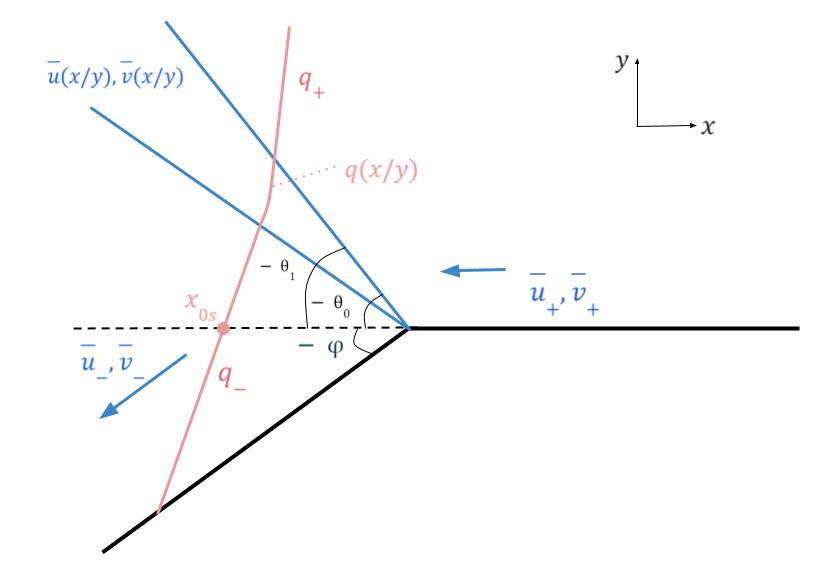
\includegraphics[width = 0.6\textwidth]{figures/KPII RW soliton interaction.jpg}
    \caption{KPII 1-wave: interaction of a soliton with rarefaction wave mean flow. Diagram is accessible and editable at \href{https://docs.google.com/drawings/d/1fx1p1iLIPBzyM74Fr5_Aun8OyIP53FncyBJjeWmVurA/edit}{\bf this link}.}
    \label{fig:KPII 1-wave}
\end{figure}

\subsubsection{1-wave} \label{sec: 1wave}


We first examine the case where $s_1 = s_1(\xi)$ and $s_2,s_3$ are constant, so that $\lambda_1 = x/y <0$ everywhere in the simple wave. For KPII, the mean flow is then negative and around a corner with a RW in the fourth quadrant. This is illustrated in Figure \ref{fig:KPII 1-wave}.

We hold $s_2,s_3$ constant and assume that $s_1 = s_1(\xi)$. Let 
\begin{align}
    s_{2,0} &= 2q_+\bar u_+ + \frac{4}{9}\sigma q_+^3 - \bar v_+ \\
    s_{3,0} &= \frac{2}{3}\sqrt{-6\sigma\bar u_+}\bar u_+ - \bar v_+
\end{align}
be the constant Riemann invariants.

Since $s_1$ is not constant with respect to $\xi$, \eqref{ode for si in xi} implies that
\begin{align}
    \lambda_1 = -\sqrt{-6\sigma\bar u} = \frac{x}{y} \label{lambda1 = x/y}
\end{align}
and thus 
\begin{align}
    \bar u(x,y) = -\frac{1}{6}\sigma\left(\frac{x}{y}\right)^2. \label{ubar1}
\end{align}
From \eqref{s3} and \eqref{lambda1 = x/y}
\begin{align}
    \bar v &= \frac{2}{3}\sqrt{-6\sigma \bar u}\bar u - s_{3,0} \nonumber\\
    &= \frac{2}{3}\left(-\frac{x}{y}\right)\left(-\frac{1}{6}\sigma\left(\frac{x}{y}\right)^2\right) - s_{3,0} \nonumber\\
    &= \frac{1}{9}\sigma\left(\frac{x}{y}\right)^3 - s_{3,0} \label{vbar1}
\end{align}
Note that \eqref{ubar1} and \eqref{vbar1} are the same as \eqref{ubar} and \eqref{vbar}. To find a self-similar solution for $q$, we set $s_2 = s_{2,0}$ and obtain the cubic
\begin{align}
    q^3-\frac{3 \zeta ^2 q}{4}+\frac{9}{4} \sigma  \left(s_{3,0}-s_{2,0}\right)-\frac{\zeta ^3}{4} &= 0, \label{cubic in q - 1-wave}
\end{align}
with discriminant
\begin{align}
    \Delta_q &= \frac{27}{16}\left(2\sigma \zeta^3 - 9(s_{3,0}-s_{2,0})\right)\cdot 9(s_{3,0}-s_{2,0}).
    \label{disc of cubic in q 1}
\end{align}
When $\Delta_q >0$, \eqref{cubic in q - 1-wave} will have three real roots.\footnote{There is no proof in this document that this will always be the case; that is, there may or may not be a situation in which $\Delta_q<0$ and only one root is real. Empirically, however, we see that analytical solutions given by the real roots match the numerical solutions.} The self-similar, stationary 1-wave solutions in the soliton limit can then be written as
\begin{align}
    \bar u(x,y) &= -\frac{1}{6}\sigma\left(\frac{x}{y}\right)^2, \;
    \bar v(x,y) = \frac{1}{9}\sigma\left(\frac{x}{y}\right)^3 - s_{3,0} \\
    q(x,y) &= \left|\frac{x}{y}\right|\cos\left[\frac{1}{3}\mathrm{arccos}\Theta(x/y) - \frac{2(k-1)\pi}{3}\right] 
\end{align}
where $k=1,2,$ or $3$ and where $-\sqrt{-6\bar u_-} \leq x/y \leq -\sqrt{-6\bar u_+}$. From section \ref{sec: disp limit}, we know that $x/y = -\sqrt{-6\bar u_-}$ and $x/y=-\sqrt{-6\bar u_+}$ mark the left and right edges of the rarefaction wave, respectively, in the KPII 1-wave case. $\bar u$, $\bar v$, and $q$ are constant elsewhere as determined by $u_+,u_-,v_+,v_-$. $\Theta$ is defined as 
\begin{align}
    \Theta(x/y) = \left|\frac{y}{x}\right|^3\left(\left(\frac{x}{y}\right)^3 - 9\sigma(s_{3,0}-s_{2,0})\right)
\end{align}
It is necessary to determine for which values of $k$ the solution is valid. \footnote{I started trying to prove this, but didn't finish.} Numerical results indicate that if $q_- <0$ (the soliton is moving to the right, as in Figure \ref{fig:KPII 1-wave}), we should choose $k=3$. If $q_- >0$ (the soliton is moving to the left, but it still interacts with the RW), we should choose $k = 1$. The 1-wave solution is then given by 
\begin{subequations}
    \begin{align}
        \bar u(x/y) &= \left\{\begin{array}{ll}
             \bar u_+ &   -\sqrt{-6\bar u_+} < x/y\\
             -\frac{1}{6}\sigma\left(\frac{x}{y}\right)^2 & -\sqrt{-6\bar u_-} \leq x/y \leq -\sqrt{-6\bar u_+} \\
             \bar u_- & x/y < -\sqrt{-6\bar u_-}
        \end{array}\right. \\
        \bar v(x/y) &= \left\{\begin{array}{ll}
              0 &   -\sqrt{-6\bar u_+} < x/y\\
             -\frac{1}{6}\sigma\left(\frac{x}{y}\right)^2 & -\sqrt{-6\bar u_-} \leq x/y \leq -\sqrt{-6\bar u_+} \\
             \bar v_- & x/y < -\sqrt{-6\bar u_-}
        \end{array}\right. \\
        q(x/y) &= \left\{\begin{array}{ll}
              q_+ &   -\sqrt{-6\bar u_+} < x/y\\
             \left|\frac{x}{y}\right|\cos\left[\frac{1}{3}\mathrm{arccos}\Theta(x/y) - \frac{4\pi}{3}\right] & -\sqrt{-6\bar u_-} \leq x/y \leq -\sqrt{-6\bar u_+}, \; q_- <0 \\
             \left|\frac{x}{y}\right|\cos\left[\frac{1}{3}\mathrm{arccos}\Theta(x/y)\right] & -\sqrt{-6\bar u_-} \leq x/y \leq -\sqrt{-6\bar u_+}, \; q_->0 \\
             q_- & x/y < -\sqrt{-6\bar u_-}
        \end{array}\right. 
    \end{align} \label{exact u,v,q}
\end{subequations}

Here $\bar u_+, \bar v_+,$ and $q_-$ are given. We could find $\bar u_-, \bar v_-$ in the same way as in the dispersionless limit, by taking $\varphi$ as given and solving for $\bar u_-, \bar v_-$ using \eqref{mucubic_kp2}.

Alternatively, we could (instead of prescribing $\varphi$) prescribe $\bar u_-, \bar v_-$ as well as $\bar u_+, \bar v_+,$ and $q_-$. The incoming and outgoing flow then completely describe the angle of expansion $\varphi$ (which can be determined by inverting \eqref{mucubic_kp2}). In fact, we can (without loss of generality) set $\bar u_- = -1$ and vary only $\bar v_-$ to change the angle of expansion.

In either case, we determing $q_+$ using continuity:
\begin{align}
    q_+ = q(-\sqrt{-6\bar u_+}).
\end{align}

\begin{comment}
\begin{theorem}
    If $q_->0$ (a leftgoing wave), then $q(\zeta)$ is uniquely given by the case when $k = 1$.
\end{theorem}
\begin{proof}
    First, note that $q_- <0$  if and only if $q(x/y) <0$ at the left edge of the RW. Since $q$ cannot change sign inside the RW,\footnote{I believe this is true because $q$ is an eigenvalue of the system, but don't have a proof.} this is the case if and only if (from \eqref{exact u,v,q}), 
\begin{align}
    &\cos\left[\frac{1}{3}\mathrm{arccos}\Theta(\zeta) - \frac{2(k-1)\pi}{3}\right] > 0 \label{cond q>0}
\end{align}
for all $\zeta$. This is equivalent to the condition
\begin{align*}
    &-\frac{\pi}{2}<\frac{1}{3}\mathrm{arccos}\Theta - \frac{2(k-1)\pi}{3} < \frac{\pi}{2}\\
    \implies &\frac{\pi}{2} + \frac{1}{3}\mathrm{arccos}\Theta > \frac{2(k-1)\pi}{3} > -\frac{\pi}{2} + \frac{1}{3}\mathrm{arccos}\Theta.  \\
\end{align*}
If $k = 1$ then \eqref{cond q>0} becomes
\begin{align*}
    -\frac{\pi}{2} + \frac{1}{3}\mathrm{arccos}\Theta < 0 < \frac{\pi}{2} + \frac{1}{3}\mathrm{arccos}\Theta
\end{align*}
which is always true. 

If $k = 3$, then \eqref{cond q>0} becomes
\begin{align*}
    -\frac{\pi}{2} + \frac{1}{3}\mathrm{arccos}\Theta < \frac{4\pi}{3} < \frac{\pi}{2} + \frac{1}{3}\mathrm{arccos}\Theta
\end{align*}
which is not possible. 

If $k = 2$ then \eqref{cond q>0} becomes
\begin{align*}
    -\frac{\pi}{2} + \frac{1}{3}\mathrm{arccos}\Theta < \frac{2\pi}{3} < \frac{\pi}{2} + \frac{1}{3}\mathrm{arccos}\Theta \label{k=2,q>0}
\end{align*}
which is possible, but only if $\mathrm{arccos}\Theta > \pi/2$; that is, $\Theta <0$.
\end{proof}
\end{comment}




\begin{figure}
    \centering
    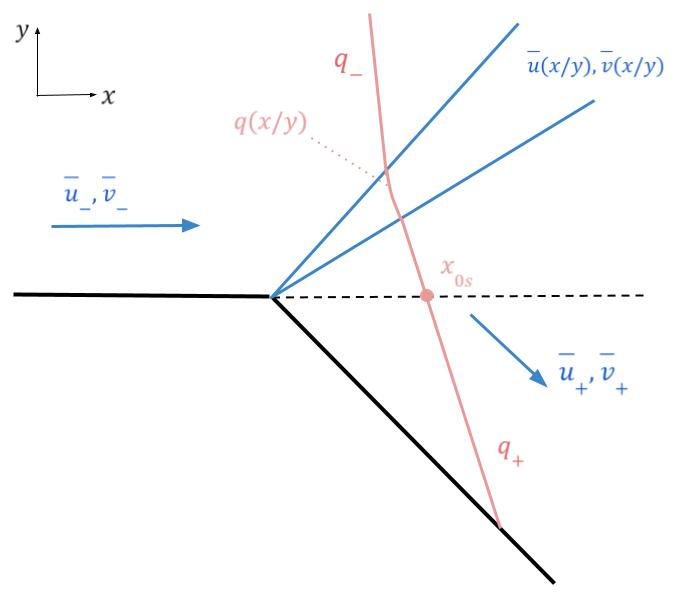
\includegraphics[width = 0.5\textwidth]{figures/KPI RW soliton interaction.jpg}
    \caption{KPI 3-wave: interaction of a soliton with rarefaction wave mean flow. Diagram is accessible and editable at \href{https://docs.google.com/drawings/d/1qAcWeN46pt7tIWzvV4KJ7gigHyIDA4orVNvBKdzfUPw/edit}{\bf this link.}}
    \label{fig:KPI 3-wave}
\end{figure}

\subsubsection{3-wave}
We next examine the case when $s_3$ is not constant, so that $\lambda_3 = x/y \geq 0$ everywhere in the simple wave. Thus the simple wave must be in the first or third quadrants. For KPI, this represents a positive mean flow around a corner with a RW in the first quadrant. This is illustrated in Figure \ref{fig:KPI 3-wave}.

We hold $s_1,s_2$ constant and assume that $s_3 = s_3(\xi)$. Let 
\begin{align}
    s_{1,0} &= -\frac{2}{3}\sqrt{-6\sigma\bar u_-}\bar u_- - \bar v_- \\
    s_{2,0} &= 2q_-\bar u_- + \frac{4}{9}\sigma q_-^3 - \bar v_- 
\end{align}
be the constant Riemann invariants. Here $\bar u_-, \bar v_-, q_-$ are the constant, given values on the left side of the KPI rarefaction wave.

Since $s_3$ is not constant with respect to $\xi$, \eqref{ode for si in xi} implies that
\begin{align}
    \lambda_3 = \sqrt{-6\sigma\bar u} = \frac{x}{y} \label{lambda3 = x/y}
\end{align}
and thus 
\begin{align}
    \bar u(x,y) = -\frac{1}{6}\sigma\left(\frac{x}{y}\right)^2. \label{ubar}
\end{align}
From \eqref{s1} and \eqref{lambda3 = x/y}
\begin{align}
    \bar v &= -\frac{2}{3}\sqrt{-6\sigma \bar u}\bar u - s_{1,0} \nonumber\\
    &= -\frac{2}{3}\left(\frac{x}{y}\right)\left(-\frac{1}{6}\sigma\left(\frac{x}{y}\right)^2\right) - s_{1,0} \nonumber\\
    &= \frac{1}{9}\sigma\left(\frac{x}{y}\right)^3 - s_{1,0} \label{vbar}
\end{align}
To obtain a self-similar solution for $q$, we set $s_2 = s_{2,0}$ and recognize that \eqref{s2} is a depressed cubic in $q$. Let $\zeta = x/y$. We can write the cubic in $q$ using $\bar u$ and $\bar v$, or using \eqref{ubar} and \eqref{vbar}.
\begin{align}
    q^3 + \frac{9}{2}\sigma \bar u q - \frac{9}{4}\sigma (\bar v + s_{2,0}) &= 0  \nonumber\\
    q^3-\frac{3 \zeta ^2 q}{4}+\frac{9}{4} \sigma  \left(s_{1,0}-s_{2,0}\right)-\frac{\zeta ^3}{4} &= 0 \label{cubic in q - 3-wave}
\end{align}

We can obtain solutions for $q$ by solving \eqref{cubic in q - 3-wave}.



\section{Harmonic limit}

As in \ref{sec: soliton limit}, we rewrite matrices \ref{a4p} and \ref{b4p} strictly in terms of $r_1,r_2,r_3$ and assume zero frequency, taking $\omega=0$. We then take the harmonic limit, $m\to 0^+$; that is, $r_2 \to r_1^+$. In doing so, the equation for $r_2$ can be eliminated, and we obtain the simplified system
\begin{align}
    A'_h\frac{\partial \textbf{r}_h}{\partial x} + B'_h \frac{\partial \textbf{r}_h}{\partial y} = 0 \label{harmpde}
\end{align} 
where $\textbf{r}_h = [r_1,r_3,p]^T$ and
\begin{subequations}
   \begin{align}
    A_h' &= \left[\begin{array}{ccc}
       16r_1-2r_3  &  r_3 & -\sqrt{2}H\sqrt{\sigma}\\
        2r_3 & 4r_1+9r_3 & -\sqrt{2}H\sqrt{\sigma} \\
        -\frac{\sqrt{2}r_3\sigma\sqrt{\sigma}}{H} & -\frac{12r_1+3r_3}{\sqrt{2}H\sqrt{\sigma}} & \sqrt{\sigma}
    \end{array}\right] \\
    B'_h &= \frac{1}{H}\left[\begin{array}{ccc}
        -\sqrt{2}(4r_1+3r_3)\sqrt{\sigma} & -\frac{r_3\sqrt{\sigma}}{\sqrt{2}} & H\sigma \\
        -\sqrt{2}r_3\sqrt{\sigma} & -\frac{(8r_1+5r_3)\sqrt{\sigma}}{\sqrt{2}} & H\sigma \\
        0 & -H & 0
    \end{array}\right]
\end{align}
\end{subequations}

with $H= \sqrt{-(2r_1+r_3)}$. 
(\ref{exactsol}), (\ref{keqxn}), (\ref{leqxn}), (\ref{qexn}) for $r_1, r_3, l,$ and $p$ with $r_2=r_1$ and $\omega=0$ to obtain
\begin{subequations}
\begin{align}
    r_1 &= -k^2\pi^2 + \bar u\\
    r_3&= \bar u\\
    p &= -\frac{\sqrt{4k^2\pi^2-6u}u}{\sqrt{\sigma}} + v \\
    l &= \frac{k\sqrt{4k^2\pi^2-6u}}{\sqrt{\sigma}}. 
\end{align} \label{toPhys}
\end{subequations}
We use the relation $l=qk$ and (\ref{toPhys}) to rewrite the latter system below: \begin{subequations}
\begin{align}
    u_y &= v_x \\
    v_y &= -6\sigma \bar u\bar u_x \\
    k_y &= l_x \\
    &= -\frac{3k}{\sqrt{\sigma}\sqrt{4\pi^2k^2-6u}}u_x + \frac{2(4\pi^2k^2-3 \bar u)}{\sqrt{\sigma}\sqrt{4k^2\pi^2-6 \bar u}}k_x.
\end{align} \label{physicalpde}
\end{subequations}
Therefore, we must transform (\ref{harmpde}) into the physical variables $u,v,$ and $k$, and then rearrange the resulting equation to solve for the partial $y$ derivatives. The transformed system is 
\begin{align}
    \frac{\partial \textbf{u}_h}{\partial y} &= -(B'J)^{-1}A'J\frac{\partial \textbf{u}_h}{\partial x} \\
    &= C'\frac{\partial \textbf{u}_h}{\partial x} \label{cprimepde}
\end{align}
where $\textbf{u}_h=[u,v,k]^T$ and $J$ is the Jacobian of the vector $\textbf{r}_h = [r_1,r_3,p]^T$. We compute $C'$ to be equal to 
\begin{align}
    C' = \left(\begin{array}{ccc}
         0 & 1 & 0  \\
         -6\sigma \bar \bar u& 0 & 0 \\
         -\frac{3k}{\sqrt{\sigma}\sqrt{4\pi^2k^2-6\bar u}} & 0 & \frac{2(4\pi^2k^2-3 \bar u)}{\sqrt{\sigma}\sqrt{4k^2\pi^2-6 \bar u}}
    \end{array}\right)
\end{align}
The system (\ref{cprimepde}) is equivalent to the system (\ref{physicalpde}), so the harmonic limit of the xy KPWS is equivalent to the dispersionless KP equation combined with the wave conservation equation.%


\subsection{Hyperbolicity and Riemann invariants}
\label{sec:hyperb-riem-invar-1}

In the harmonic limit of the stationary KPWS, our system is 
\begin{align}
    \frac{\partial v}{\partial y} = \left(
\begin{array}{ccc}
 0 & 1 & 0 \\
 -6 \sigma \bar u & 0 & 0 \\
 -\frac{3 k}{\sqrt{2} \sqrt{\sigma} \sqrt{2 \pi ^2 k^2-3 \bar u}} & 0 & \frac{\sqrt{2} \left(4 \pi ^2 k^2-3
   \bar u\right)}{\sqrt{\sigma} \sqrt{2 \pi ^2 k^2-3 \bar u}} \\ \label{harmonicpde}
\end{array}
\right) \frac{\partial v}{\partial x}
\end{align}
where $v = [\bar u, \bar v, k]^T$. Letting the matrix in (\ref{harmonicpde}) be denoted $C'_h$, we rewrite the above system $$u_y+(-C_h')u_x=0.$$ The eigenvalues of $-C'_h$ are 
\begin{align}
    \lambda_{1} = -\sqrt{-6\sigma \bar u}, \; \lambda_2 = -\frac{\sqrt{2} \left(4 \pi ^2 k^2-3
   \bar u\right)}{ \sqrt{\sigma(2 \pi ^2 k^2-3 \bar u)}}, \; \lambda_3 = \sqrt{-6\sigma \bar u}
\end{align}
The left eigenvectors are \AG{Add right eigenvectors}
\begin{align}
    \ell_{1} = \left(\begin{array}{c}
         \mp \sqrt{-6\sigma \bar u}  \\
         -1 \\
         0
    \end{array}\right), \;
    \ell_2 =\left(
\begin{array}{c}
 \frac{12k^2\pi^2-9\bar u}{4k\pi^2(-8k^2\pi^2 + 9\bar u)} \\
 -\frac{3\sqrt{\sigma(2k^2\pi^2-3 \bar u)}}{4k\pi^2\sqrt{2}(8k^2\pi^2-9\bar u) } \\
 1
\end{array}
\right).
\end{align}
We rescale $\ell_2$ as follows:
\begin{align}
    \ell_3 = \left(
\begin{array}{c}
 \frac{-(12k^2\pi^2-9\bar u)}{3\sqrt{2k^2\pi^2-3\bar u}} \\
 -\sqrt{\sigma} \\
 \frac{4\sqrt{2}k\pi^2(8k^2\pi^2-9\bar u)}{3\sqrt{2k^2\pi^2-3\bar u}}
\end{array}
\right).
\end{align}
To ensure $\lambda_1,\lambda_3 \in \Bbb R$ for hyperbolicity we require $-\sigma u \geq 0$, or 
\begin{subequations}
    \begin{align}
    \bar u &\geq 0 \text{ for } \sigma = -1\label{l13cond-1} \\
    \bar u & \leq 0 \text{ for } \sigma = 1 \label{l13cond1}
    \end{align} \label{ucond}
\end{subequations}
(for strict hyperbolicity, we require the above to be strict inequalities). To ensure $\lambda_2 \in \Bbb R$, we require
\begin{align*}
    \sigma(2 \pi^2k^2-3\bar u) > 0 \implies \sigma \bar u < \frac{2}{3}\sigma \pi^2k^2
\end{align*}
or 
\begin{subequations}
    \begin{align}
        \bar u &>\frac{2}{3}\pi^2k^2  \text{ for } \sigma = -1 \label{l2cond-1}\\
        \bar u &< \frac{2}{3}\pi^2k^2  \text{ for } \sigma = 1 \label{l2cond1}
    \end{align}
\end{subequations}
\eqref{l2cond-1} is a stronger condition than \eqref{l13cond-1}, while \eqref{l2cond1} is a weaker condition than \eqref{l13cond1}. That is, KP I $(\sigma = -1)$ loses hyperbolicity for $0 < \bar u \leq 2\pi^2k^2/3$. We also check for a loss of strict hyperbolicity in the case that $\lambda_2 = \lambda_1$ or $\lambda_2=\lambda_3$. In that case,
\begin{align*}
    \mp \sqrt{6\sigma \bar u } &= -\frac{\sqrt{2} \left(4 \pi ^2 k^2-3
   \bar u\right)}{ \sqrt{\sigma(2 \pi ^2 k^2-3 \bar u)}} \\
   -6\sigma \bar u &= \frac{2 \left(4 \pi ^2 k^2-3
   \bar u\right)^2}{\sigma(2 \pi ^2 k^2-3 \bar u)} \\
   -3\bar u (2\pi^2k^2 - 3\bar u ) &= 2(16\pi^4k^4-24\pi^2k^2\bar u + 9 \bar u ^2) \\
   18\pi^2k^2\bar u &= 16\pi^4k^4 \\9\bar u &= 8\pi^2k^2
\end{align*}
Thus for strict hyperbolicity we require $\bar u \neq 8\pi^2k^2/9$. This falls in the region of hyperbolicity for the case $\sigma = -1$, but not for the case $\sigma = 1$.\\
\\
Now we find the Riemann invariants; from the eigenvalues and left eigenvectors, we obtain differential equations for the Riemann invariants $s_{1,2,3}$:
\begin{subequations}
\begin{align}
    \d s_{1} &= -\sqrt{-6\sigma \bar u} \d \bar u - \d \bar v = 0 \label{riemanndiffharm1} \\
    \d s_2 &= \frac{-(12k^2\pi^2-9\bar u)}{3\sqrt{2k^2\pi^2-3\bar u}}\d \bar u -\sqrt{\sigma}\d \bar v + \frac{4\sqrt{2}k\pi^2(8k^2\pi^2-9\bar u)}{3\sqrt{2k^2\pi^2-3\bar u}} \d k = 0 \label{riemanndiffharm2} \\
     \d s_{3} &= \sqrt{-6\sigma \bar u} \d \bar u - \d \bar v = 0 \label{riemanndiffharm3} 
\end{align}
\end{subequations}
Equations (\ref{riemanndiffharm1}) and (\ref{riemanndiffharm2}) are easily integrable, and (\ref{riemanndiffharm2}) can be written in the form $d\left(F(\bar u,k) - \sqrt{\sigma}\bar v \right)$. We find the function $F$,
\begin{align}
    F_{\bar u }(\bar u, k) &= \frac{-(12k^2\pi^2-9\bar u)}{3\sqrt{2k^2\pi^2-3\bar u}} \\
    F(\bar u, k) &= \frac{2}{9} \sqrt{2 \pi ^2 k^2-3 \bar u} \left(8 \pi ^2 k^2-3 \bar u\right) + \psi(k)
\end{align}
where $\psi$ is an unknown function of $k$. Taking the derivative with respect to $k$ and equating to the coefficient of $\d k$ in (\ref{riemanndiffharm2}), we have 
\begin{align}
    F_k(\bar u, k) &= \frac{4 \sqrt{2} \pi ^2 k \left(8 \pi ^2 k^2-9 \bar u\right)}{3 \sqrt{2 \pi ^2 k^2-3 \bar u}} + \psi'(k) = \frac{4 \sqrt{2} \pi ^2 k \left(8 \pi ^2 k^2-9 \bar u\right)}{3 \sqrt{2 \pi ^2 k^2-3 \bar u}}.
\end{align}
We conclude that $\psi'(k)=0$, and choose $\psi(k)=0$. Integrating (\ref{riemanndiffharm1})-(\ref{riemanndiffharm3}), we obtain the Riemann invariants for the harmonic KPWS,
\begin{subequations}
\begin{align}
    s_{1} &= -\sqrt{-6\sigma}\cdot \frac{2}{3}\bar u^{3/2} - \bar v \\
    s_2 &= \frac{2}{9} \sqrt{2 \pi ^2 k^2-3 \bar u} \left(8 \pi ^2 k^2-3 \bar u\right) - \sqrt{\sigma}\bar v \\
     s_{3} &= \sqrt{-6\sigma}\cdot \frac{2}{3}\bar u^{3/2} - \bar v.
\end{align}
\end{subequations}

The right eigenvectors for the harmonic limit of the stationary KPWS are 
\begin{align}
    r_{1,3} &= \left(
\begin{array}{c}
 \frac{2 \left(\mp\sqrt{3} \sqrt{- \bar u \left(2 \pi ^2 k^2-3 \bar u\right)}+4 \pi ^2 k^2-3 \bar u\right)}{3 k} \\
  \frac{2 \sqrt{2\sigma} \left(2 \pi ^2 k^2 \left(2 \sqrt{9 \bar u^2-6 \pi ^2 k^2 \bar u}\pm3 \bar u\right)-3 \bar u
   \left(\sqrt{9 \bar u^2-6 \pi ^2 k^2 \bar u}\mp3 \bar u\right)\right)}{3 k \sqrt{2 \pi ^2 k^2-3 \bar u}} \\
   1 \\
\end{array}
\right), r_2 = \left(\begin{array}{c}
     0 \\
     0 \\
     1 
\end{array}\right)
\end{align}
with eigenvalues
\begin{align}
    \lambda_{1} = -\sqrt{-6\sigma \bar u}, \; \lambda_2 = -\frac{\sqrt{2} \left(4 \pi ^2 k^2-3
   \bar u\right)}{ \sqrt{\sigma(2 \pi ^2 k^2-3 \bar u)}}, \; \lambda_3 = \sqrt{-6\sigma \bar u}
\end{align}
For linear degeneracy, we require $\nabla \lambda_j \cdot r_j = 0 $ for some $j \in \{1,2,3\}$. For $j = 1,3$,
\begin{align*}
    0 &= \mp \sqrt{\frac{6\sigma}{\bar u}}\cdot \frac{8\pi^2k^2-6\bar u \mp 2\sqrt{-6k^2\pi^2\bar u + 9 \bar u ^2}}{3k} \\
     0 &= 4k^2\pi^2-3\bar u \mp \sqrt{-6k^2\pi^2\bar u + 9 \bar u ^2}
\end{align*}
which gives the condition 
\begin{align}
    \bar u = \frac{8}{9}k^2 \pi ^2. \label{nonlinearity condition}
\end{align}
In particular, genuine nonlinearity will be lost when when $\nabla\lambda_1 \cdot r_1 = 0$, since we require $8\pi^2k^2-6\bar u k>0$, or $\bar u < \frac{8}{6}k^2\pi^2$ for the above condition to hold in that case. We find that $\nabla\lambda_3 \cdot r_3 = 0$ only when $4k^2\pi^2-3\bar u <0$, which implies $\bar u > \frac{8}{6}k^2\pi^2$. Since $8/6>8/9$, this will not occur.\\
\\
Note that \eqref{nonlinearity condition} is also the curve along which strict hyperbolicity is lost ($\lambda_1=\lambda_2$), in the $\sigma = -1$ case.

For $j= 2$, genuine nonlinearity is lost ($\nabla \lambda_2 \cdot r_2=0$) if 
\begin{align}
    0=\frac{2 \sqrt{2} \pi ^2 k \left(9 \bar u-4 \pi ^2 k^2\right)}{\sqrt{\sigma} \left(2 \pi ^2 k^2-3 \bar u\right)^{3/2}}
\end{align}
which occurs when 
\begin{align}
    \bar u &= \frac{4}{9}\pi^2k^2.\label{nonlinearity condition 2}
\end{align}

\section{Numerical Results}
In this section we discuss the numerical solution to the good Boussinesq equation, which (from section \ref{sec: equiv to bouss}) is equivalent to finding solutions of the steady KPII equation. We discuss the mechanics of the numerical scheme, the error of the scheme, and include some comparison with analytical results.

\subsection{Numerical scheme: Boussinesq\_RK4\_Riemann}
This is a brief description of the numerical solver for the Boussinesq equation. The code is \texttt{Boussinesq\_RK4\_Riemann}. It should be able to integrate any boundary conditions, including solitons and Riemann conditions, and combinations of the two. We take the good Boussinesq equation from \eqref{good boussinesq},
\begin{align}
    U_{tt} - U_{xx} + (U^2)_{xx}  + U_{xxxx} &= 0 \label{good boussinesq}
\end{align}
and define the new dependent variable $\tilde{W} = U_x$. We take one derivative in $x$ and take $U_x \to \tilde{W}$. This gives the equation
\begin{align}
    \tilde{W}_{tt} - \tilde{W}_{xx} + 2 (U \tilde{W})_{xx} + \tilde{W}_{xxxx} = 0
\end{align}
We now define the dependent variable $\tilde{V}$ such that $\tilde{V}_x = \tilde{W}_t$. Note that since $\tilde{V}_{xx} = \tilde{W}_{tx} =U_{xxt}$, we can integrate twice in $x$ to obtain $\tilde{V} = U_t$. With $\tilde{W}$ and $\tilde{V}$, we have the system 
\begin{subequations}
    \begin{align}
        \tilde{W}_t &= \tilde{V}_x \\
        \tilde{V}_t &= \tilde{W}_{x} + 2(U\tilde{W})_{x} + \tilde{W}_{xxx}
    \end{align} \label{bouss system in w and v}
\end{subequations} 
we then implement a spectral integrating factor Runge-Kutta-4 method on the interval $[-L,L]$ for \eqref{bouss system in w and v}, using the formula 
\begin{align}
     U(x,t) &= \sum_{n \neq 0} \frac{\hat{\tilde{W}}_n(t)}{ik_n}e^{ik_nx} - \frac{1}{2L}\int_{-L}^Lx\tilde{W}(x,t)\dd x  + (x+L)\frac{U_+-U_-}{2L} + U_- . \label{equation B.6}
\end{align}
where $U_- = U(-L,t)$ and $U_+ = U(L,t)$ to find the antiderivative $\int \tilde{W} \dd x = U$ at each step. The implementation is 
\begin{align}
    U(x_j,t) \approx \mathcal{F}^{-1}\left( \ldots \hat{\tilde{W}}_{-2},\hat{\tilde{W}}_{-1}, - \sum_{j=-N/2}^{N/2-1}x_j\tilde{W}(x_j,t), \hat{\tilde{W}}_1, \hat{\tilde{W}}_2, \ldots \right) + (x_j+L)\frac{U_+-U_-}{2L} + U_-, \label{numerical approx of u from w=u_x}
\end{align}
where $x_j = \frac{2L}{N}j$. In \eqref{numerical approx of u from w=u_x} the integral from \eqref{equation B.6} is evaluated using the trapezoidal rule.

\subsection{Soliton/RW boundary conditions}
Exact soliton solutions to the stationary KPII equation (\eqref{statKP}, $\sigma =1$) are given by 
\begin{align}
    u(x,y) = \bar u + a\sech^2\left(\sqrt{\frac{a}{2}}(x-x_0+qy)\right)
\end{align}
where $a$ must satisfy the condition \eqref{a(q)}. Exact soliton solutions to gBq \eqref{good boussinesq} are given by 
\begin{align}
    U(x,t) &= \bar U + A\sech^2\left(\sqrt{\frac{A}{6}}\left(x-x_0 - Ct\right)\right)
\end{align}
where 
\begin{align}
    C = \pm \sqrt{-2\bar U + 1 - 2A/3} \label{C}
\end{align}
and $\bar U = 3\bar u + \frac{1}{2}$ and $A = 3a$. Here $\bar U$ is the mean flow and $A$ is the soliton amplitude. We obtain the constraint \eqref{C} from \eqref{a(q)} and the equivalence in section \eqref{sec: equiv to bouss}.

In order to numerically model the interaction of a soliton with a rarefaction wave, we combine soliton and Riemann initial conditions. The analytical solution in this case is given by the KPII 1-wave soliton solution in section \ref{sec: 1wave}.

That is, we want to numerically evaluate \eqref{good boussinesq} with the initial condition
\begin{align}
    U(x,0) = A\sech^2\left(\sqrt{\frac{A}{6}}(x-x_0)\right) + \left\{
    \begin{array}{cc}
        u_- & x<x_0 \\
        u_+ & x\geq x_0
    \end{array}\right. \label{exact initial cond}
\end{align}
Originally, I smoothed and implemented \eqref{exact initial cond} via the initial conditions
\begin{subequations}
    \begin{align}
         U(x,0) =& A\sech^2\left(\sqrt{\frac{A}{6}}(x-x_0)\right) + \frac{1}{2}\left(\tanh\left(-B(x-x_0)\right) + 1\right)(U_--U_+) + U_+ \\
          \tilde{W}(x,0) =& -\sqrt{\frac{2}{3}}A^{3/2}\sech^2\left(\sqrt{\frac{A}{6}}(x-x_0)\right)\mathrm{tanh}\left(\sqrt{\frac{A}{6}}(x-x_0)\right) \nonumber \\
          & -\frac{B}{2}\sech^2\left(-B(x-x_0)\right)(U_--U_+) \\
        \tilde{V}(x,0) =& \sqrt{\frac{2}{3}}CA^{3/2}\sech^2\left(\sqrt{\frac{A}{6}}(x-x_0)\right)\mathrm{tanh}\left(\sqrt{\frac{A}{6}}(x-x_0)\right) \nonumber \\
          & -\frac{B}{2}\sech^2\left(-B(x-x_0)\right)(V_- -V_+) 
    \end{align} \label{old initial cond}
\end{subequations}
where $V_{\pm} = V(\pm L,0)$, and $V$ is defined as in \eqref{boussinesq evolution}. That is, $V_x = U_t = \tilde{V}$. It is useful to use $V$ because it directly corresponds to the stationary KPII solutions; that is, $V = 3v$, where $v$ is defined as in \eqref{steady KP evolution}. Thus $V_{\pm}$ represent the incoming and outgoing flow in the $y$ direction.

Using \eqref{old initial cond} results in numerical error - a kind of "extra" soliton that propagates in the opposite direction as the "main" soliton.

In order to prevent this error, we need to use the constant Riemann invariant $s_3$ to determine $\tilde{V}(x,0)$, rather than finding it exactly as in \eqref{old initial cond}. For reference, the characteristic velocities for the steady KP soliton limit are
    \begin{align}
        \lambda_1 = -\sqrt{-6\sigma \bar u}, \hspace{3mm}
        \lambda_2 = -q, \hspace{3mm}
        \lambda_3 = \sqrt{-6\sigma \bar u}
        \end{align}
and the Riemann invariants are
    \begin{align}
        s_{1} = -\frac{2}{3}\sqrt{-6\sigma \bar u}\bar u - \bar v, \hspace{3mm}
        s_{2}= 2q\bar u + \frac{4}{9}\sigma q^3 - \bar v, \hspace{3mm}
        s_{3} = \frac{2}{3}\sqrt{-6\sigma \bar u}\bar u - \bar v.
    \end{align}

(This is the same as in section \ref{sec:sol char velocities and riemann inv}, but included for reference). To obtain the soliton/RW interaction for steady KPII in the soliton limit, we take $\sigma = 1$ and assume $s_3 = s_{3,0}$ and $s_2 = s_{2,0}$ are constant. We can then use $s_3$ to determine the Riemann condition part of $\tilde{V}(x,0)$.

Then 
\begin{align*}
    \bar v(x,0) &= \frac{2}{3}\sqrt{-6\bar u(x,0)}\bar u (x,0) - s_{3,0} \\
    \tilde{V}(x,0)
    &= 3\cdot \bar v_x(x,0)\\
    &= 3\cdot \frac{2}{3}\left[\frac{1}{2}(-6\bar u(x,0))^{-1/2}(-6\bar u_x(x,0))\bar u(x,0) + \sqrt{-6\bar u(x,0)}\bar u_x(x,0)\right]
\end{align*}
Combining this with the soliton initial conditions, we can use
\begin{subequations}
    \begin{align}
         U(x,0) =& A\sech^2\left(\sqrt{\frac{A}{6}}(x-x_{0sol})\right) + \frac{1}{2}\left(\tanh\left(-B(x-x_0)\right) + 1\right)(U_--U_+) + U_+ \\
          \tilde{W}(x,0) =& -\sqrt{\frac{2}{3}}A^{3/2}\sech^2\left(\sqrt{\frac{A}{6}}(x-x_{0sol})\right)\mathrm{tanh}\left(\sqrt{\frac{A}{6}}(x-x_{0sol})\right) \nonumber \\
          & -\frac{B}{2}\sech^2\left(-B(x-x_0)\right)(U_--U_+) \\
        \tilde{V}(x,0) =& \sqrt{\frac{2}{3}}CA^{3/2}\sech^2\left(\sqrt{\frac{A}{6}}(x-x_0)\right)\mathrm{tanh}\left(\sqrt{\frac{A}{6}}(x-x_0)\right) \nonumber \\
          & + 2\left[\frac{1}{2}(-6\bar u(x,0))^{-1/2}(-6\bar u_x(x,0))\bar u(x,0) + \sqrt{-6\bar u(x,0)}\bar u_x(x,0)\right]
    \end{align} \label{soliton/RW initial cond}
\end{subequations}
where 
\begin{align}
    \bar u(x,0) &= \frac{1}{3}U(x,0) = \frac{1}{3}\left(\frac{1}{2}\left(\tanh\left(-B(x-x_0)\right) + 1\right)(U_--U_+) + U_+\right) \\
    \bar u_x(x,0) &= \frac{1}{3}\tilde{W}(x,0) = \frac{1}{3}\cdot -\sqrt{\frac{2}{3}}A^{3/2}\sech^2\left(\sqrt{\frac{A}{6}}(x-x_{0sol})\right)\mathrm{tanh}\left(\sqrt{\frac{A}{6}}(x-x_{0sol})\right)
\end{align}


\subsection{Error analysis}
We an evaluate the accuracy of the method by comparing to the exact soliton solution
\begin{align}
    U(x,t) = \bar U + A\sech^2\left(\sqrt{\frac{A}{6}}(x-x_0-Ct)\right), \hspace{3mm} C = \pm \sqrt{-2\bar U +1-\frac{2}{3}A} \label{soliton exact solution}
\end{align}
where $1/C$ is the slope of the soliton trajectory, $A$ is the amplitude, and $\bar u_B$ is the background. This is an exact solution of the good Boussinesq equation, verified in Mathematica. The correct initial conditions for $w$ and $v$ are then 
\begin{subequations}
    \begin{align}
        \tilde{W}(x,0) = U_x(x,0) &= -\sqrt{\frac{2}{3}}A^{3/2}\sech^2\left(\sqrt{\frac{A}{6}}(x-x_0)\right)\mathrm{tanh}\left(\sqrt{\frac{A}{6}}(x-x_0)\right) \\
        \tilde{V}(x,0) = U_t(x,0) &= \sqrt{\frac{2}{3}}CA^{3/2}\sech^2\left(\sqrt{\frac{A}{6}}(x-x_0)\right)\mathrm{tanh}\left(\sqrt{\frac{A}{6}}(x-x_0)\right)
    \end{align} \label{initial cond w and v}
\end{subequations} 
Figure \ref{fig:riemann soliton} shows the error in the numerical solution to the Boussinesq equation for a soliton with zero background. We see a saturation at around $10^{-11}$ for $\Delta t = 10^{-3}$ and $N \geq 2^9$.

\begin{figure}
     \centering
     \begin{subfigure}[b]{.45\textwidth}
        \centering
        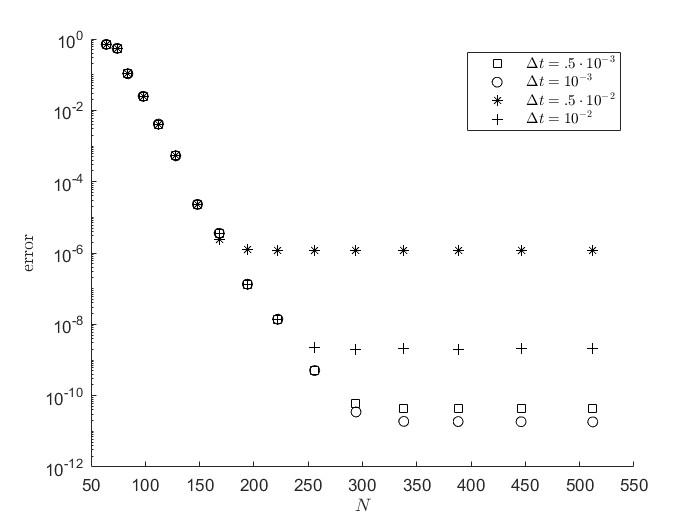
\includegraphics[width = \textwidth]{figures/errorbyN_Riemann_soliton.jpg}
         \caption{}
     \end{subfigure}
     \hfill
     \begin{subfigure}[b]{.45\textwidth}
        \centering
        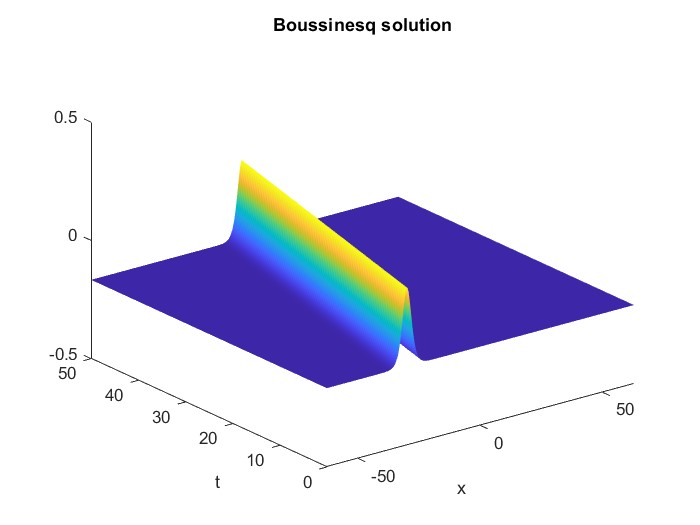
\includegraphics[width = \textwidth]{figures/soliton_single_bouss.jpg}
         \caption{}
     \end{subfigure}
        \caption{(a) error in numerical solutions (b) example of numerical solution with soliton initial conditions given by \eqref{initial cond w and v} with $A = 1$, $x_0 = -30$, $\bar U = u_-=u_+ = 0$, and $C>0$.}
        \label{fig:riemann soliton}
\end{figure}


\subsection{Comparison with analytical results}
We can integrate the boundary conditions \eqref{soliton/RW initial cond} and compare with the exact analytical solution, given by 



\begin{figure}[h!]
     \centering
     \begin{subfigure}[b]{.45\textwidth}
        \centering
        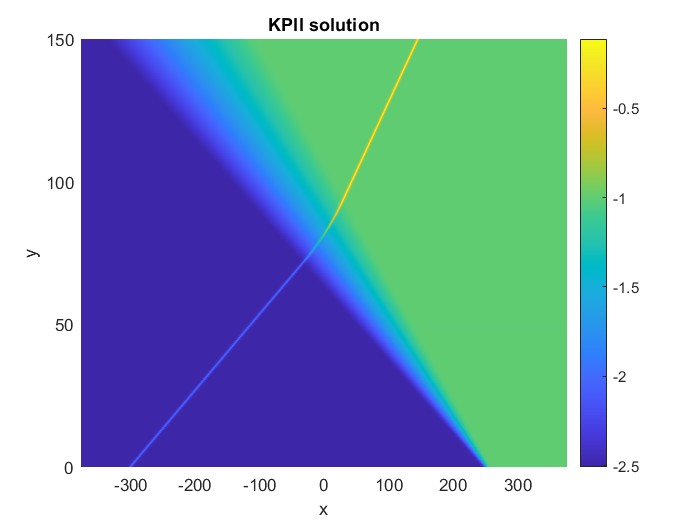
\includegraphics[width = \textwidth]{figures/KPII_RWsoliton_above_good.jpg}
         \caption{}
     \end{subfigure}
     \hfill
     \begin{subfigure}[b]{.45\textwidth}
        \centering
        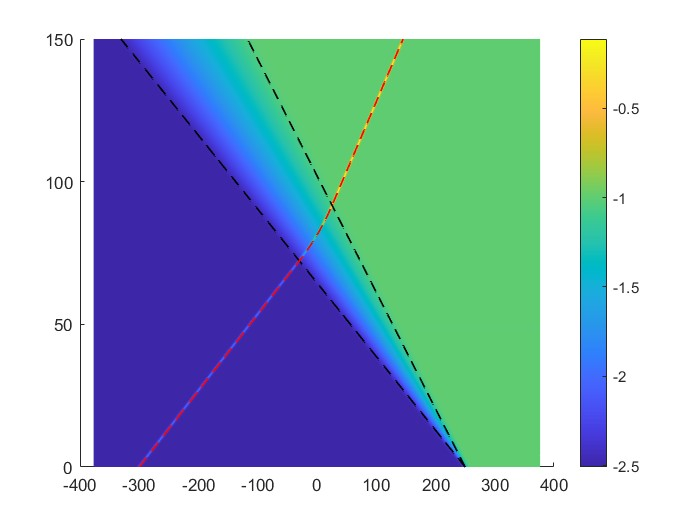
\includegraphics[width = \textwidth]{figures/RWsolitoncomp.jpg}
         \caption{}
     \end{subfigure}
        \caption{\textbf{(a)} Interaction of a soliton with a rarefaction wave. The initial parameters are $a = 1/2$, $u_+ = - 1$, $u_- = -5/2$, ($A = 3/2$, $U_+ = -5/2$, $U_- = -7$). The soliton's initial location is $x_{0sol} = -300$ and the RW's initial location is $x_0 = 250$. The shaping parameter for the tanh function is $B = 0.3$. Other parameters: $N = 2^{11}$, $\Delta t = 5\times10^{-3}$. \textbf{(b)} Comparison to analytical solution (dashed line).} 
        \label{fig:comparison narrower}
\end{figure}

\begin{figure}[h!]
     \centering
     \begin{subfigure}[b]{.45\textwidth}
        \centering
        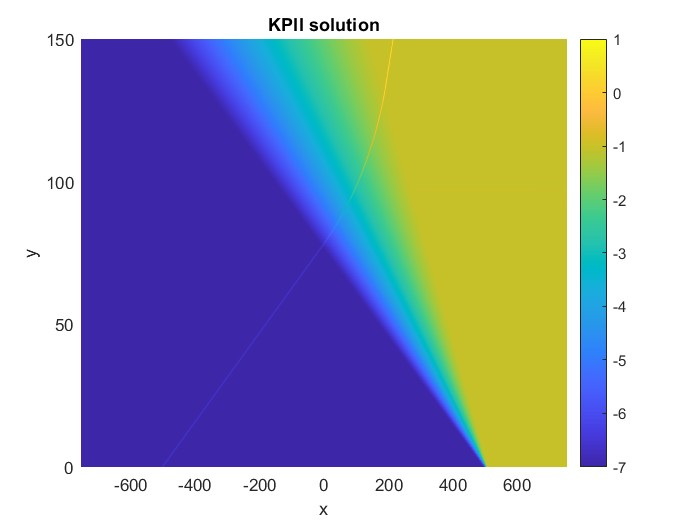
\includegraphics[width = \textwidth]{figures/KPIIsolitonRW2.jpg}
         \caption{}
     \end{subfigure}
     \hfill
     \begin{subfigure}[b]{.45\textwidth}
        \centering
        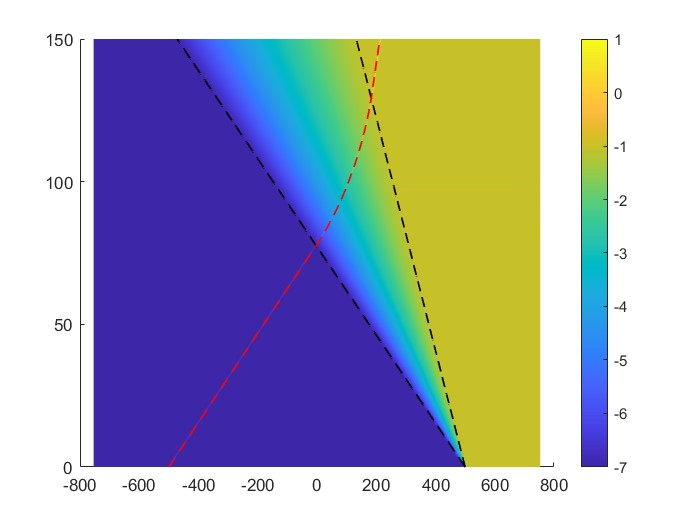
\includegraphics[width = \textwidth]{figures/KPIIsolitonRW2_comp.jpg}
         \caption{}
     \end{subfigure}
        \caption{\textbf{(a) }Interaction of a soliton with a rarefaction wave. The initial parameters are $a_- = 1/2$, $u_+ = - 1$, $u_- = -7$, ($A = 3/2$, $U_+ = -5/2$, $U_- = -7$). The soliton's initial location is $x_{0sol} = -500$ and the RW's initial location is $x_0 = 500$. The shaping parameter for the tanh function is $B = 0.3$. Other parameters: $N = 2^{12}$, $\Delta t = 5\times10^{-3}$. \textbf{(b)} Comparison to analytical solution (dashed line).} 
        \label{fig:comparison wider}
\end{figure}

\pagebreak

\bibliographystyle{unsrt}
\bibliography{refs}

\end{document}
